%!TEX root = ../masters_thesis.tex

\chapter{Development} % (fold)
\label{cha:development}

This thesis aims for a comphrehensive Historical Geographic Information System. The previous chapter has shown that this is a very complicated undertaking, because both the reality and the human using the system are complex. For such complex applications the methodologies of \emph{Human Centered Design} are promising to create an interface that humans can easily understand.

The development process is iterative and divided in several phases. The outcome of each phase is a prototype of the interface that gets closer to the desired solution by increasing the fidelity of the prototype. A phase starts with an initial set of requirements. In multiple iterations, a prototype is developed that solves the problem. Each iteration has four steps: The requirements for the system are analyzed in the \emph{planning} step. Afterwards, they translated into an abstract \emph{design} which is realized in a specific \emph{implementation} of the prototype. Finally, this prototype is tested with humans to find out how well it works. Based on the results of this \emph{testing} step, the requirements are updated and the next iteration starts. This is repeated until a version of the interface is created that sufficiently solves the problem. Then the fidelity is increased, starting the next development phase. The five phases in this thesis are shown in figure \ref{fig:human_centered_design}.

\begin{figure}[H]
  \vspace{1em}
  \centering
  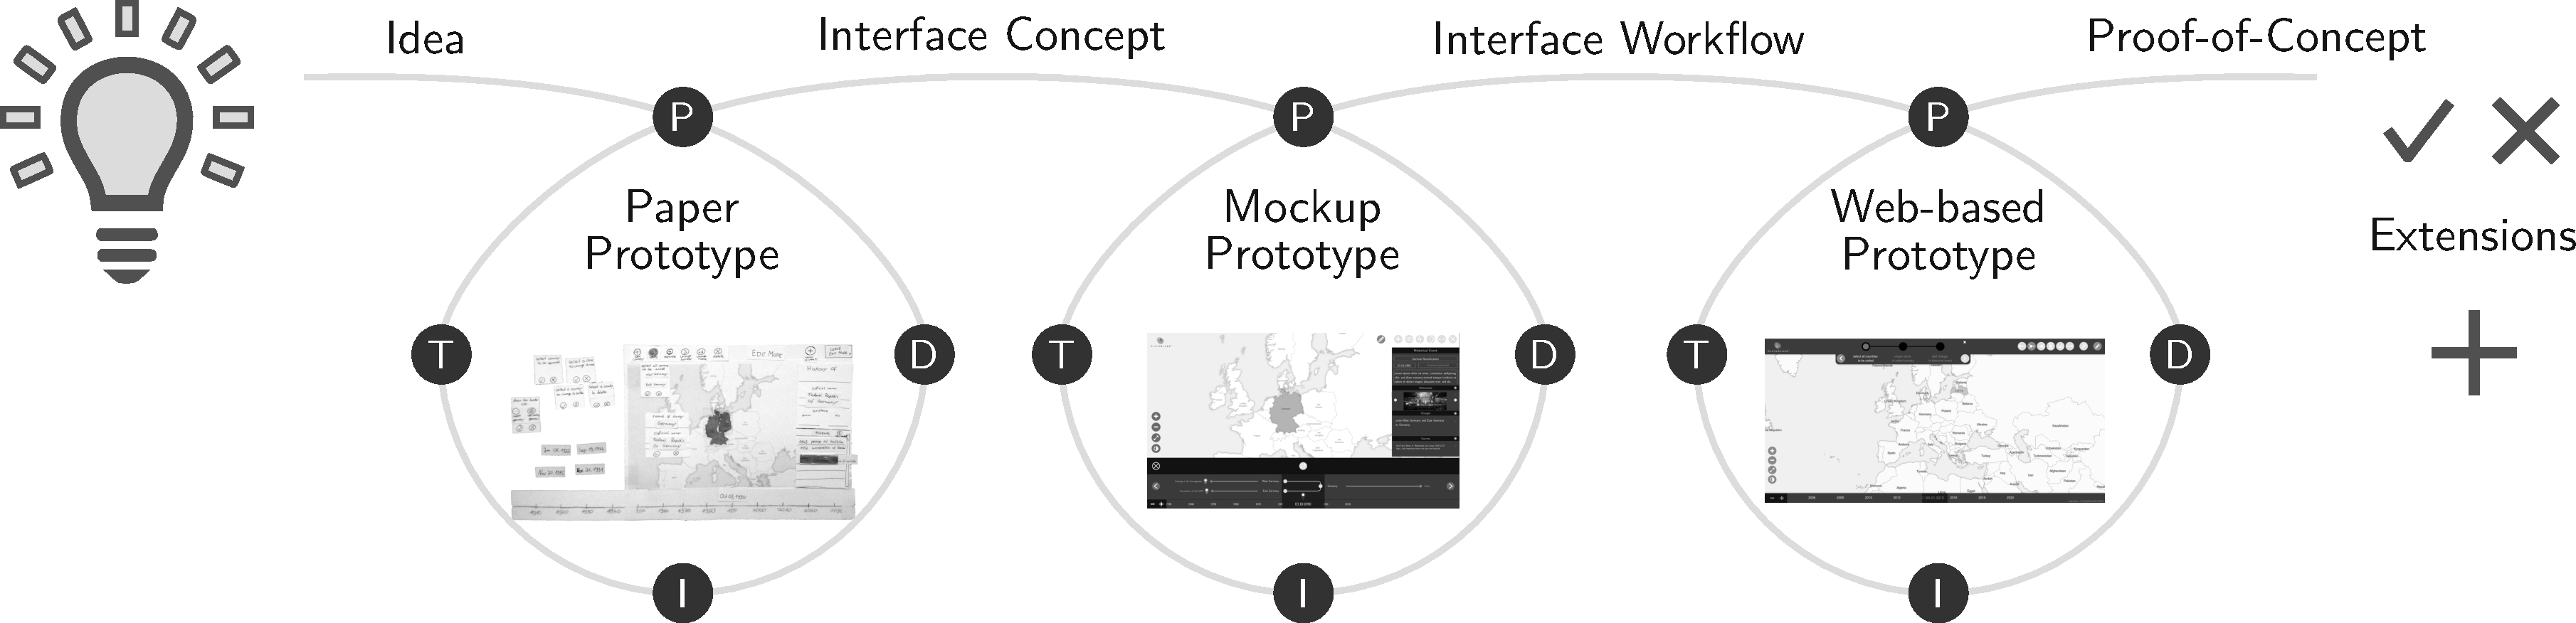
\includegraphics[width=0.9\textwidth]{graphics/development/human_centered_design}
  \caption{Human Centered Design process with five project phases}
  \label{fig:human_centered_design}
\end{figure}

\newpage
\begin{compactenum}
  \item \textbf{Idea}: The initial idea how to edit and visualize the history of countries.
  \item \textbf{Paper prototype}: The concept of the interface realized and tested on paper.
  \item \textbf{Mockup prototype}: The concrete workflow developed in a slide-based presentation.
  \item \textbf{Web-based prototype}: The final version developed in a Web application.
  \item \textbf{Extensions}: Design approaches to account for the uncertain nature of history.
\end{compactenum}

This chapter covers the first four phases of this design process, focusing on the results of the Web-based prototype and its underlying data model. Everything in this chapter is based on the assumption of full certainty about the data: For each time point in history there a clear an undisputed state of the world. The data model and the application presented in this chapter is be open to extension to tackle the actual problem of uncertainty in history. This is the topic of the next chapter \ref{cha:uncertainty}.

\begin{figure}[H]
  \vspace{1.5em}
  \centering
  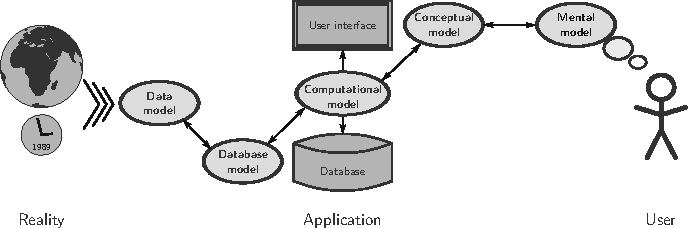
\includegraphics[width=0.8\textwidth]{graphics/development/models}
  \caption{Relevant models for an information system}
  \label{fig:models}
\end{figure}

There are several models involved in the development of the software. The \emph{data model} is an abstraction and simplification of the real world. The \emph{Hivent Model} developed in this thesis is explained in the first section \ref{sec:hivent_model} of this chapter. It is followed by section \ref{sec:editing_hivent_data} with methods to \emph{edit} the spatio-temporal data in the system. In iteractive computer systems, the \emph{mental model} is the representation in the mind of the human about how the interface should work -- the \emph{conceptual model} describes the way the interface actually works. The goal of Human Centered Design is to match the conceptual model to the mental model. Section \ref{sec:user_interface_design_process} outlines the gradual design process to reach this goal. In the application, the data model is implemented in the \emph{database model}. The task for the \emph{computational model} is to translate between the database model and the conceptual model. The implementation of HistoGlobe including the latter three models is presented in the last section \ref{sec:application} of this chapter.

% ==============================================================================
\newpage
%!TEX root = ../masters_thesis.tex

\section{Hivent Model} % (fold)
\label{sec:hivent_model}

This section proposes the spatio-temporal \emph{Hivent model} to represent countries and their evolution in time and space. In section \ref{sec:spatio_temporal_data_models}, different spatio-temporal data models were introduced. The \emph{Snapshot Model} is unsuitable for the problem space. \emph{Simple Time-Stamping} is helpful to link countries to their history, but it does not explicitly model historical changes, which is desireable. For that purpose, the idea of the \emph{Event-Based Spatio-Temporal Data Model} was developed, but since it only works for raster data, it is also not suitable for this thesis. This problem is solved in the \emph{History Graph Model}. Additionally, the introduced temporal changes allow to represent historical changes and their influences on geographic entities directly in the model. Finally, the \emph{Three-Domain Model} introduces a helpful concept to separate the spatial, temporal and thematic dimension of a spatio-temporal entity.

The Hivent Model is constructed from components of some of these models: It is event-based and supports vector data. It is organized in four domains and allows to visualize data on a graph. The first section \ref{sub:elements} introduces the main elements of the Hivent model. Afterwards, the preconditions are defined in section \ref{sub:preconditions}. One major contribution of this thesis is proposed in section \ref{sub:hivent_operations}: the set of five \emph{Hivent Operations} that describe all possible changes of countries in time and space. This section closes with the \emph{HistoGraph} (section \ref{sub:histograph}), a visualization of the evolution of countries.

% ------------------------------------------------------------------------------
\subsection{Elements} % (fold)
\label{sub:elements}

% - - - - - - - - - - - - - - - - - - - - - - - - - - - - - - - - - - - - - - -
\vspace{-1em}
\paragraph{Hivents} % (fold)
\label{par:hivent}

represent historically significant happenings, e.g. a treaty, bill or declaration.
The word is an acronym for \emph{\textbf{Hi}}storical e\emph{\textbf{vent}}.
The focus in this work is on events that influence the geopolitical situation on Earth.
An Hivent happens at one particular point in time and space and is therefore the main organizing elements of the eponymic data model.

% paragraph hivent (end)

% - - - - - - - - - - - - - - - - - - - - - - - - - - - - - - - - - - - - - - -
\vspace{-1em}
\paragraph{Areas} % (fold)
\label{par:area}

represent one identical current or historical country. They are an abstract entity on the map with a \emph{name} and a \emph{territory}. The name consists of a common \emph{short name}, e.g. ``Germany'' and a \emph{formal name}, e.g. ``Federal Republic of Germany''. The \emph{territory} of the Area is described by a polypolygon, a set of weakly simple polygons to support enclaves and exclaves. The polylines of a polygon consist of an ordered set of points that represent a border of the country. They are either \emph{interior}, i.e. bordering another country, or a \emph{coastline}, bordering a body of water. Additionally, an Area keeps a reference to the historical changes creating, updating and ceasing it.

% paragraph area (end)

% ------------------------------------------------------------------------------
\vspace{-1em}
\paragraph{Historical Changes} % (fold)
\label{par:historical_changes}

influence the evolution of Areas over time. Throughout the lifetime of an Area, it is created at some point $t_s$, then its territory and short name can change multiple times $t_i: t_s < t_i$ and at some point $t_e: t_s < t_i < t_e$ it ceases. Since all changes in this model are sudden, there are only two possible states an Area can be in: It is \emph{active}, if at the current time point it is historically existing and it is \emph{inactive} if it does not. Each Area is \textbf{uniquely identified by its formal name}. That means as soon as the formal name of an Area changes (e.g. ``German Empire'' to ``Federal Republic of Germany''), it is considered a ``new'' Area. Each Historical Change belongs to exactly one Hivent, inheriting its time point at which the change happens.  The change is described by a Hivent Operation introduced in section \ref{sub:hivent_operations}.

\begin{figure}[H]
  \vspace{1em}
  \centering
  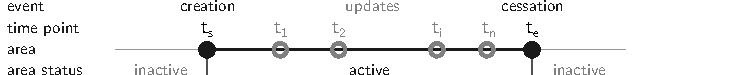
\includegraphics[width=0.9\textwidth]{graphics/development/area_states}
  \caption{Three event types that change Areas, resulting in two different area states}
  \label{fig:area_states}
\end{figure}


% paragraph historical_changes (end)

% subsection section area (end)

% ------------------------------------------------------------------------------
\subsection{Preconditions} % (fold)
\label{sub:preconditions}

\begin{quoteit}
In the beginning God created the heavens and the Earth \\
Now the Earth was formless and empty [...] \\
And God said, “Let there be light” --- and there was light.
\end{quoteit}
\vspace{-1em}
\hfill -- Genesis 1:1, The First Book of Moses, Old Testament

There are five axoims and two assumptions the Hivent Model is based on. The theoretical foundation is the model of the Earth and its curved surface that can be projected on a two-dimensional map using a map projection, as introduced in sections \ref{sub:model_of_geographical_space}.

\vspace{-1.0em}
\newtheorem{invariant_surface}[assicounter]{Axiom}
\begin{invariant_surface}
\label{axm:invariant_surface}
  The Earth's surface has an invariant area size, i.e. it does not change over time.
\end{invariant_surface}

\vspace{-2.5em}
\newtheorem{area_on_surface}[assicounter]{Axiom}
\begin{area_on_surface}
\label{axm:area_on_surface}
  Each Area in the spatio-temporal system is located directly on the surface of the Earth.
\end{area_on_surface}

These axiom sets the spatial foundation of the system: a constant dimension of the map and Areas covering the map. The basis of the temporal part of the system is content of the next three axioms:

\vspace{-1.0em}
\newtheorem{initial_configuration}[assicounter]{Axiom}
\begin{initial_configuration}
\label{axm:initial_configuration}
  The spatio-temporal system has an initial state at time point $t_0$. At this initial state, there exists exactly one Area, denoted by $\Omega$ and referred to as the \emph{universe} Area. It has no name and its territory covers the whole surface of the Earth.
\end{initial_configuration}

\vspace{-2.5em}
\newtheorem{historical_change}[assicounter]{Axiom}
\begin{historical_change}
\label{axm:historical_change}
  At each time point $t_i \geq t_0$ multiple historical changes can be introduced.
\end{historical_change}

\vspace{-2.5em}
\newtheorem{unique_coverage}[assicounter]{Axiom}
\begin{unique_coverage}
\label{axm:unique_coverage}
  At each time point $t_i \geq t_0$ each point on the surface of the Earth is covered by exactly one territory of exactly one Area.
\end{unique_coverage}

As it has been defined in section \ref{par:historical_changes}, an Historical Change can create, manipulate and cease Areas on the Earth's surface. According to axoim \ref{axm:unique_coverage}, each change introduced in the system must maintain the spatial integrity on the map: When an Area with a territory is created on the map, the Area claiming this territory before has to cease it. Formally, it can be said that each change consists of a set of old Areas $A$ that are manipulated, a set of new Areas $B$ that are created in the change, and an operation $\rightarrow_C$ describing the change. Each Area $A_i \in A$ and $B_i \in B$ has a territory $A_i^T$  respectively $B_i^T$. For each change introduced in the system, the territories of the old Areas must have the same size than the territories of the new Areas to maintain the spatial integrity of axiom \ref{axm:unique_coverage}:
\begin{align*}
  \bigcup\limits_{i=1}^n A_i^T ~\textbf{=}~ \bigcup\limits_{i=1}^n B_i^T
\end{align*}

The first changes introduced in the system at time point $t_0$ are the creation of all bodies of water, including the oceans and lakes, denoted as $W$. Each Area $W_i \in W$ is created with their name and territory cut out of $\Omega$. The result is that after $t_0$, the map is divided into water ($W$) and land ($\Omega$). Land can at any point in time be either \emph{claimed}, i.e. it is currently occupied by the territory of exactly one active Area, or on a contrary be \emph{unclaimed}, i.e. belonging to $\Omega$. It is a subtractive data model, because each new Areas territory is cut out of $\Omega$.

\begin{figure}[H]
  \centering
  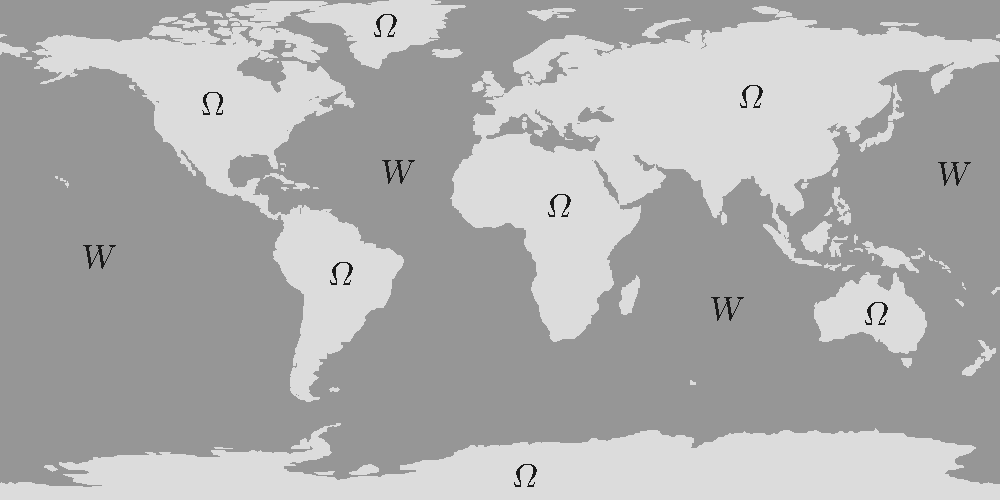
\includegraphics[width=0.5\textwidth]{graphics/development/init_map}
  \caption{The initial state of the world map at time point $t_0$}
  \label{fig:init_map}
\end{figure}

In the real world, the name of a country changes according to sudden events, e.g. a declaration or a governmental bill. The territory can change either because of a geographical processes, e.g. the sea level rise influencing the change of the coastline, or according to a historical event, e.g. a treaty. The Hivent model is based on two assumptions that simplify the model and keep the problem space clear:

\vspace{-1.0em}
\newtheorem{coastline_territory}[assicounter]{Assumption}
\begin{coastline_territory}
\label{axm:coastline_territory}
  The territory of a country stops at the coastline.
\end{coastline_territory}

\vspace{-2.0em}
\newtheorem{constant_coastlines}[assicounter]{Assumption}
\begin{constant_coastlines}
\label{axm:constant_coastlines}
  The spatial configuration of water and the coastlines have not changed over time.
\end{constant_coastlines}

Both assumptions are obviously wrong: In line with \cite{UNSeaBorders}, the territory of a country extends in a range of 3 to 12 miles (5 to 20 kilometers) into international waters. They are constantly changing and so does the distribution of land and water on Earth. However, the assumptions allow the Hivent Model to focus only on discrete historical changes. It is subject to future work to extend the data model to account for long-term processes that change water and the coastlines. For now, the temporal behavior of an Area in the Hivent Model can be described as a \emph{static object that changes according to sudden events}.

% base: Newtons concept of absolute space?
% TODO: topological rule?
% each border has exactly two neighboring Areas
% each Area has at least one neighboring Area

% subsection preconditions (end)

% ------------------------------------------------------------------------------
\subsection{Hivent Operations} % (fold)
\label{sub:hivent_operations}

Respecting the preconditions, there are several different types of changes that transform a set of old Areas $A$ to a set of new Areas $B$. All possible changes can be expressed with only five spatio-temporal operations that are called \emph{Hivent Operations}. The first four change the identity of a set of Areas and therefore establish historical predecessor-successor-relationships. They are always symmetric, i.e. if one old Area is replaced by one new Area, the old Area is the historical predecessor of the new Area and vice versa the new Area is the successor of the old Area. The last operation changes an aspatial property of an Area.

\begin{description}

  \item[UNI -- Unification]
  A set of old Areas unifies to one new Area. The old Areas cease, becoming the historical predecessors of the new Area. The territory of this new Area is the union of the territories of the old Areas. The new Area receives a new name. \\[0.25em]
  \begin{footnotesize}
    In 1922, the Russian SFSR, the Transcaucasian SFSR, the Ukrainian SSR and the Byelorussian SSR unified and formed the Union of Soviet Socialist Republics (USSR).
  \end{footnotesize}

  \item[INC -- Incorporation]
  One or more old Areas are incorporated into another Area that stays active. Its territory is enlarged by the union of the territories of the old Areas. The old Areas are historical predecessors of the Area that stays active. \\[0.25em]
  \begin{footnotesize}
    In 1990, the territory of the German Democratic Republic (East Germany) became part of the Federal Republic of Germany (West Germany). Although this event is known as the \emph{German Reunification}, it is historically an incorporation of East Germany into West Germany \cite{incorporationEastWestGermany}.
  \end{footnotesize}

  \item[SEP -- Separation]
  As the inverse of unification, one old Area is separated into multiple new Areas. Each new Area gets a part of the territory of the old Area, receives a new name, and has the old Area as its only historical predecessor. \\[0.25em]
  \begin{footnotesize}
    In 1993, the Czech and Slovak Federal Republic, commonly known as Czechoslovakia, dissolved into present-day Czech Republic and Solvak Republic, creating two new countries out of one old.
  \end{footnotesize}

  \item[SEC -- Secession]
  As the inverse of incorporation, one or more new Areas are ceded from a previously existing Area that stays active. Each new Area gets a new name, receives the previously existing Area as the only historical predecessor and a part of its territory. \\[0.25em]
  \begin{footnotesize}
    In 2008, the Republic of Kosovo declared independence from Serbia and has since then partially received international recognition. Serbia stays a country, keeping its name, but ceding a part of its territory to Kosovo.
  \end{footnotesize}

  \item[NCH -- Name Change]
  An Area changes its short name but preserves its formal name and identity. \\[0.25em]
  \begin{footnotesize}
    A recent change happened on 5. May 2016: The cabinet of Czech Republic approved that the country will now offically be called ``Czechia''. However, the formal name stays ``Czech Republic'', which preserves its identity.
  \end{footnotesize}
\end{description}

\vspace{1.5em}
\begin{table}[H]
\begin{center}
\begin{tabular}{cx{2.5cm} cx{2.5cm} cx{2.5cm} cx{2.5cm} cx{2.5cm}}

  \toprule
  \texttt{UNI} & \texttt{INC} & \texttt{SEP} & \texttt{SEC} & \texttt{NCH} \\
  Unification & Incorporation & Separation & Secession & Name Change \\[1em]

  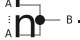
\includegraphics{graphics/development/hivent_operations/UNI} &
  
\includegraphics{graphics/development/hivent_operations/INC} &
  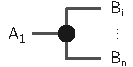
\includegraphics{graphics/development/hivent_operations/SEP} &
  
\includegraphics{graphics/development/hivent_operations/SEC} &
  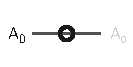
\includegraphics{graphics/development/hivent_operations/NCH} \\

  \bottomrule
\end{tabular}
\caption{The five Hivent Operations}
\label{tab:hivent_operations}
\end{center}
\end{table}

% subsection hivent_operations (end)

% ------------------------------------------------------------------------------
\subsection{HistoGraph} % (fold)
\label{sub:histograph}

Based on the idea of the History Graph Model (section \ref{fig:history_graph_model}), the linguistically and conceptually related \emph{HistoGraph} visualizes the evolution of countries in time, without any spatial relation. The edges of the graph represent an Area, the nodes a Hivent Operation. The graph shows the predecessor-successor-relationships between Areas. This is easily possible, because in the Hivent Model an Area keeps references to the historical changes creating, updating and ceasing the Area (section \ref{par:area}).

The two-dimensional HistoGraph has an horizontal orientation. The x-axis refers to one time point, the y-axis has no spatio-temporal relation and depends how much space it needs. The graph uses the visualization approach of the five Hivent Operations (table \ref{tab:hivent_operations}), including the following symbols:

\begin{table}[H]
\begin{center}
\begin{tabular}{c l l}

  \raisebox{3.5\height}
  {
\includegraphics{graphics/development/histograph/line}}
  & Area
  & \\

  \raisebox{-0.2\height}
  {
\includegraphics{graphics/development/histograph/circle_filled}}
  & Identity-changing Hivent Operation
  & \texttt{UNI}, \texttt{INC}, \texttt{SEP}, \texttt{SEC} \\

  \raisebox{-0.2\height}
  {
\includegraphics{graphics/development/histograph/circle_unfilled}}
  & Property-changing Hivent Operation
  & \texttt{NCH} \\

  \raisebox{-0.2\height}
  {
\includegraphics{graphics/development/histograph/circle_combo}}
  & A combination of both
  & e.g. \texttt{INC + NCH}

\end{tabular}
\label{tab:histograph_symbols}
\end{center}
\end{table}

\vspace{-2em}

Each uninterrupted horizontal line refers to exactly one Area. If an horizontal line leads straight through a circle, the identity of the Area is preserved in the operation. New Areas resulting from an identity-changing Hivent Operation emerge from the circle with a vertical line, indicating a sudden change with zero duration. From this line, the new Areas branch out right-angled. The HistoGraph is created from one particular reference Area. It visualizes historically related Areas in one direction: into the past, it recursively plots the predecessors on the graph, but not the predecessors successors. Into the future, the successors of the reference Area are plotted recursively, but not their predecessors.

The behavior of the HistoGraph is shown in figure \ref{fig:example_germany} at the example of present-day Germany and its state history since the end of World War II. This history is driven by six historical events, which provide examples for all five Hivent Operations. They are listed in table \ref{tab:german_history_since_1945}.

\begin{figure}[ht]
  \vspace{0.5em}
  \centering
  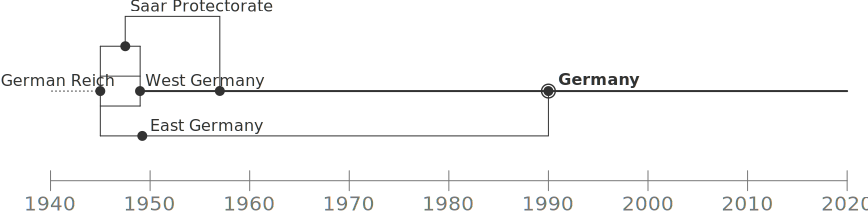
\includegraphics[width=0.8\textwidth]{graphics/development/histograph/example_germany}
  \caption{The concept of the HistoGraph at the example of the history of Germany since 1945}
  \label{fig:example_germany}
\end{figure}


\begin{table}[ht]
\begin{center}
\begin{tabular}{l p{8.5cm} l}
  \toprule
  Hivent date & Hivent description & Hivent Operations \\
  \midrule

    05.06.1945
  & \footnotesize{In the Berlin Declaration the total dissolution of the Third Reich is confirmed. It separates into multiple parts, returning the territories annexed by the German Reich in World War II. The rest is controlled by the British, French, American and Soviet occupation zone.}
  & \texttt{SEP} \\

    16.02.1946
  & \footnotesize{The Saar Protectorate is entangled from the French Zone of Occupation Germany, creating an own country.}
  & \texttt{SEC} \\

    28.05.1949
  & \footnotesize{The Federal Republic of Germany (West Germany) is created from the British, American and French Zone of Occupation.}
  & \texttt{UNI} \\

    07.10.1949
  & \footnotesize{The German Democratic Republic (East Germany) is created from the Soviet Zone of Occupation.}
  & \texttt{UNI} \\

    01.01.1957
  & \footnotesize{The Saar Treaty (``Little Reunification'') joins the Saar Protectorate as the Bundesland Saarland in West Germany.}
  & \texttt{INC} \\

    03.10.1990
  & \footnotesize{In the German Reunification, East Germany joins West Germany. The Federal Republic of Germany is now just called ``Germany''.}
  & \texttt{INC + NCH} \\

  \bottomrule
\end{tabular}
\caption{Historical events in German state history since 1945}
\label{tab:german_history_since_1945}
\end{center}
\end{table}

The example hosts a special case: in October 1949, East Germany was created from the Soviet Zone of Occupation. Both Areas have the same territory, but a different short and formal name. A \texttt{NCH} can not be performed, because the identity is not preserved: The German Democratic Republic is a new Area. However, the change can be described by a \texttt{UNI} of only one Area (Soviet zone), creating a new Area (East Germany) and establishing a historical relationship between both.

The graph plots Germany first. Since it does not have any successors, the plot goes only one way, historically backwards: East Germany and the Saar Protectorate were incorporated into Germany, so they are plotted. They emerged from the four post-war occupation zones, visualized next. All of the four occupation zones themselves originated from the German Reich. However, the Reich dissolved into many more Areas, e.g. the Memel territory. They are not included in the graph, because they are not predecessors of any Area that is a recursive predecessor of present-day Germany.

Many problems of the graph visualization are apparent in this example: Circles my overlap, if many operations happen in a short period of time -- in this case between 1945 and 1949.
The name ``West Germany'' collides with the vertical line indicating the incorporation of the Saar Protectorate, which should also be avoided.
Additionally, the names of the Areas of the four post-war occupation zones can not be shown in the graph, because there is no space for them.
One more important aspect can be seen in the creation of West Germany in 1949: A \texttt{UNI} operation unifies three old Areas to one new Area. This could be visualized symmetrically with a straight line from the midmost incoming Area line into the circle to the outgoing Area line of the new Area. This would give the wrong impression that this midmost Area has the same identity than the newly created Area. In general, the circle for \texttt{UNI} and \texttt{SEP} operations with an odd number of old respectively new Areas must be displaced off the center to emphasize that the identity has changed.
All these issues are not in the scope of this thesis and subject to future work in the field of Information Visualization.

% subsection histograph (end)

% section hivent_model (end)
%!TEX root = ../masters_thesis.tex

\section{Editing Hivent Data} % (fold)
\label{sec:editing_hivent_data}

The previous section proposed the abstract Hivent Model, a set of Hivent operations and a visualization method. However, one purpose of the HGIS developed in this thesis is to add, alter and delete historical changes. This section presents the tools and methods to edit spatio-temporal data about the development of Areas in the Hivent Model. Whereas the Hivent Operations are well-defined and specific, user studies have shown that they are not well understood by humans to edit Areas. This thesis therefore introduces a different set of six \emph{Edit Operations} in section \ref{sub:edit_operations}. Afterwards, section \ref{sub:edit_workflow} shows a \emph{workflow} to perform an Edit Operation step by step. The Hivent Model needs to support editing historical changes in between other historical changes. The last section \ref{sub:retrospective_updates} explains the theoretical approach to \emph{retrospecitve updates} of spatio-temporal data in the Hivent Model.

% ------------------------------------------------------------------------------
\subsection{Edit Operations} % (fold)
\label{sub:edit_operations}

The Hivent Operations are valuable, because they can describe all possible changes in the development of Areas in time and space. They are really well understood from the system point of view and form the basis for the Hivent Model. However, one purpose of the HGIS developed in this thesis is to provide a well understood user interface to edit historical changes to Areas.

Throughout the development process, interviews with researchers in humanities at University of Virginia were conducted to understand their mental model about the task. It turned out that the Hivent Operations are not suitable to be used for human edit purposes, because of their low-level nature. One example is that the operations do not provide a straightforward way to create a new Area on previously unclaimed land. The same is true for changing the formal name of an Area. Therefore, this thesis introduces a second set of operations: five high-level \emph{Edit Operations} describe changes to countries on the map (see table \ref{tab:edit_operations}). They have proven to be understandable in several user studies.

\vspace{0.5em}
\begin{table}[H]
\begin{center}
\begin{tabular}{m{0.75cm} m{0.8cm} m{2.4cm} m{9.1cm}}
  \raisebox{-0.35\height}
  {
\includegraphics[width=0.72cm]{graphics/development/editing_hivent_data/edit_operations/CRE}} &
  \texttt{CRE} & Create &
  a new Area with a new name and territory on the map. \\

  \raisebox{-0.35\height}
  {
\includegraphics[width=0.72cm]{graphics/development/editing_hivent_data/edit_operations/MRG}} &
  \texttt{MRG} & Merge &
  two or more Areas to a new Area. The name has to be set manually, the territory is automatically unified. \\

  \raisebox{-0.35\height}
  {
\includegraphics[width=0.72cm]{graphics/development/editing_hivent_data/edit_operations/DIS}} &
  \texttt{DIS} & Dissolve &
  one Area into two or more new Areas, manually setting their new territory and name. \\

  \raisebox{-0.35\height}
  {
\includegraphics[width=0.72cm]{graphics/development/editing_hivent_data/edit_operations/CHB}} &
  \texttt{CHB} & Change Borders &
  between two neighboring Areas by defining the territory that changes sides. \\

  \raisebox{-0.35\height}
  {
\includegraphics[width=0.72cm]{graphics/development/editing_hivent_data/edit_operations/REN}} &
  \texttt{REN} & Rename &
  an Area and set a new formal name, short name or both. \\

  \vspace{0.35em}
  \raisebox{-0.35\height}
  {
\includegraphics[width=0.72cm]{graphics/development/editing_hivent_data/edit_operations/CES}} &
  \texttt{CES} & Cease &
  an Area by deleting it from the map, leaving unclaimed land. \\

\end{tabular}
\caption{The six Edit Operations}
\label{tab:edit_operations}
\end{center}
\end{table}

% - - - - - - - - - - - - - - - - - - - - - - - - - - - - - - - - - - - - - - -
\paragraph{Error correction} % (fold)
\label{par:error_correction}

Another possible use case for the HGIS created in this thesis is to correct wrong information in the system. For this purpose it is important to understand how correcting information in an event-based spatio-temporal system works: Given time point $t_y$ and an Area $A$ with the name $X$. If $X$ happens to be wrong, it means that the historical change at time point $t_x: t_x < t_y$ that created the name $X$ for Area $A$ is erroneous and has be corrected. Correcting a state means correcting the operation that created this state.

% paragraph error_correction (end)

% subsection edit_operations (end)

% ------------------------------------------------------------------------------
\subsection{Edit Workflow} % (fold)
\label{sub:edit_workflow}

An Edit Operation describes an historical change that can be understood and performed by a user of the HGIS. This section shows that each Edit Operation can be internally expressed by a set of Hivent Operations. Therefore the Edit Operations are an abstraction layer in the Hivent Model between the Hivent and the Hivent Operations. To create an Edit Operation, four steps in a workflow need to be performed:

\begin{compactenum}
  \item Select the Areas that will be changed in the Edit Operation.
  \item For each new Area resulting from the Edit Operation, create a territory.
  \item For each new Area create a name.
  \item Add the Edit Operation to an Hivent to inherit the time point.
\end{compactenum}

For each Edit Operation, the requirements for the steps are different. Not all operations need all steps, because some data can be processed automatically. Table \ref{tab:editoperations_in_worklow} presents an overview about the behavior of the Edit Operations in the first three steps. The last step is necessary for all.

\begin{table}[H]
\begin{center}
\begin{tabular}{m{0.9cm} m{4.2cm} m{4.2cm} m{3.5cm}}
  \toprule

  &
  \emph{Select old Areas} &
  \emph{Create new territories} &
  \emph{Create new names} \\

  \midrule
  \texttt{CRE} &
  -- &
  create a territory of the new country &
  create a name for the new country \\

  \midrule
  \texttt{MRG} &
  select the countries to be merged &
  \pbox{4.4cm}{--\\
  \footnotesize{territories of selected countries are automatically unified}} &
  create a name for the new country
  \\

  \midrule
  \texttt{DIS} &
  select a country to be \mbox{dissolved} &
  create a territory for each new country &
  create a name for each new country \\

  \midrule
  \texttt{CHB} &
  select two neighboring countries to change their border &
  \pbox{4.4cm}{create the new border between both countries \\
  \footnotesize{the territory for both countries will be created automatically}}  &
  -- \\

  \midrule
  \texttt{REN} &
  select a country to rename it &
  -- &
  create a new name of the country \\

  \midrule
  \texttt{CES} &
  select a country to cease it &
  -- &
  -- \\

  \bottomrule
\end{tabular}
\caption{The requirements of each step for the Edit Operations}
\label{tab:editoperations_in_worklow}
\end{center}
\end{table}

% - - - - - - - - - - - - - - - - - - - - - - - - - - - - - - - - - - - - - - -

% wording:
% UNI of "[old]"  to    "new"
% INC of "[old]"  into  "pres"
% SEP of "old"    into  "[new]"
% SEC of "[new]"  from  "pres"
% NCH of "pres"

\vspace{-1.0em}

Depending on the input of the user in the steps for an Edit Operation, there are different possibilities to express it by a set of Hivent Operations. Each Hivent Operation transforms a set of old Areas into a set of new Areas and can update the name or territory of one specific Area. All possibilities are introduced in table \ref{tab:editoperations_to_hg_operations}. Hivent Operations are combined when they happen at the same time. In the example of the German Reunification, East Germany was incorporated into West Germany which at the same time changed its short name to ``Germany'' (\texttt{INC + NCH}).

\begin{center}
\begin{longtable}{m{1.2cm} m{0.95cm} m{0.95cm} m{0.95cm} m{6.0cm} m{2.3cm}}
  \toprule

  \pbox{1.2cm}{EditOp.\\(case)} &
  \pbox{0.95cm}{old\\Areas\\[-0.8em]} &
  \pbox{0.95cm}{update\\Areas\\[-0.8em]} &
  \pbox{0.95cm}{new\\Areas\\[-0.8em]} &
  expression by Hivent Operations \protect\footnotemark &
  visualization \\
  \midrule
  \endhead

  % TODO: introduce T as territory that is used like a temporary Area with exactly that territoy

  %%% CREATE %%

  \multirow{9}{*}{\texttt{CRE} (1)} &
  \multicolumn{4}{p{10cm}}{
    Area $B_1$ is created with territory $T$. The part of $T$ that is on previously unclaimed land ($T_\Omega$) is seceded as $B_1$ from $\Omega$.
    If $T_\Omega$ is empty, then $B_1$ is initialized with an empty territory.
    The rest of $T$ covers some Areas $A_p$ partially and some Areas $A_f$ fully.
    For each $A_p$, the covered territory $T_p$ is seceded and incorporated into $B_1$.
    Each $A_f$ is completely incorporated into $B_1$.
  } &
  \multirow{9}{*}{
    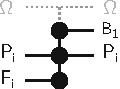
\includegraphics[width=2.5cm]{graphics/development/editing_hivent_data/edit_to_hivent_operations/CRE_to_SEC+UNI}
  } \\

  &
  $n_f$ &
  $n_p$ &
  $1$ &
  \pbox{6.0cm}{
    ~\\
    \texttt{SEC} of $B_1$ from $\Omega$ \\
    \texttt{SEC} of $T_p$ from $A_p$, \texttt{INC} of $T_p$ into $B_1$ \\
    \texttt{INC} of $A_f$ into $B_1$
  } &
  \\

  %%% MERGE %%

  \midrule
  \multirow{3}{*}{\texttt{MRG} (1)} &
  \multicolumn{4}{p{10cm}}{
    Multiple Areas $A_i$ are unified to $B_1$. The new Area receives a name distinct from all the names of $A_i$.
  } &
  \multirow{3}{*}{
    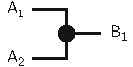
\includegraphics[width=2.5cm]{graphics/development/editing_hivent_data/edit_to_hivent_operations/MRG_to_UNI}
  } \\
  &
  $n \geq 2$ &
  $0$ &
  $1$ &
  \pbox{6.0cm}{
    \texttt{UNI} of $\forall A_i$ to $B_1$
  } &
  \\

  \midrule
  \multirow{4}{*}{\texttt{MRG} (2)} &
  \multicolumn{4}{p{10cm}}{
    Multiple Areas $A_i$ are unified. The resulting Area reuses the short and formal name of one of the old Areas ($A_0$) and therefore preserves it. The remaining Areas $A_i$ are incorporated into $A_0$.
  } &
  \multirow{4}{*}{
    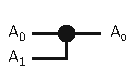
\includegraphics[width=2.5cm]{graphics/development/editing_hivent_data/edit_to_hivent_operations/MRG_to_INC}
  } \\
  &
  $n \geq 1$ &
  $1$ &
  $1$ &
  \pbox{6.0cm}{
    \texttt{INC} of $\forall A_i$ into $A_0$
  } &
  \\

  \midrule
  \multirow{4}{*}{\texttt{MRG} (3)} &
  \multicolumn{4}{p{10cm}}{
    The same as the previous case, just that $A_0$ receives a new short name and therefore an additional name change is required.
  } &
  \multirow{4}{*}{
    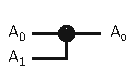
\includegraphics[width=2.5cm]{graphics/development/editing_hivent_data/edit_to_hivent_operations/MRG_to_INC+NCH}
  } \\
  &
  $n \geq 1$ &
  $1$ &
  $1$ &
  \pbox{6.0cm}{
    ~\\
    \texttt{INC} of $\forall A_i$ into $A_0$ \\
    \texttt{NCH} of $A_0$
  } &
  \\

  %%% DISSOLVE %%

  \midrule
  \multirow{4}{*}{\texttt{DIS} (1)} &
  \multicolumn{4}{p{10cm}}{
    Multiple Areas $B_i$ are separated from one initial Area $A_0$. Each $B_i$ receives a part of the territory of $A_0$ and a name. Each name is distinct from the name of $A_0$.
  } &
  \multirow{4}{*}{
    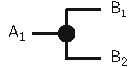
\includegraphics[width=2.5cm]{graphics/development/editing_hivent_data/edit_to_hivent_operations/DIS_to_SEP}
  } \\
  &
  $1$ &
  $0$ &
  $n \geq 1$ &
  \pbox{6.0cm}{
    ~\\
    \texttt{SEP} of $A_1$ into $\forall B_i$
  } &
  \\

  \midrule
  \multirow{5}{*}{\texttt{DIS} (2)} &
  \multicolumn{4}{p{10cm}}{
    Multiple Areas $B_i$ are separated from one initial Area $A_0$. Each $B_i$ receives a part of the territory of $A_0$ and a name. One of the separated Areas has the same short and formal name as $A_0$, so it preserves its identity. The remaining new Areas secede from $A_0$.
  } &
  \multirow{5}{*}{
    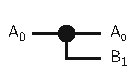
\includegraphics[width=2.5cm]{graphics/development/editing_hivent_data/edit_to_hivent_operations/DIS_to_SEC}
  } \\
  &
  $1$ &
  $1$ &
  $n \geq 1$ &
  \pbox{6.0cm}{
    ~\\
    \texttt{SEC} of $\forall B_i$ from $A_0$
  } &
  \\

  \midrule
  \multirow{4}{*}{\texttt{DIS} (3)} &
  \multicolumn{4}{p{10cm}}{
    The same as the previous case, just that $A_0$ receives a new short name and therefore an additional name change is required.
  } &
  \multirow{4}{*}{
    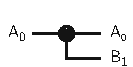
\includegraphics[width=2.5cm]{graphics/development/editing_hivent_data/edit_to_hivent_operations/DIS_to_SEC+NCH}
  } \\
  &
  $1$ &
  $1$ &
  $n \geq 1$ &
  \pbox{6.0cm}{
    ~\\
    \texttt{SEC} of $\forall B_i$ from $A_0$  \\
    \texttt{NCH} of $A_p$
  } &
  \\

  %%% CHANGE BORDER %%%

  \midrule
  \multirow{10}{*}{\texttt{CHB} (1)} &
  \multicolumn{4}{p{10cm}}{
    One existing Area $A_0$ is selected and its territory changes. Relative to the old territory some parts of the territory expands ($T_e$) and some withdraws ($T_w$).
    The part of $T_e$ that expands into unclaimed land ($T_\Omega: T_\Omega \in T_e$) is seceded from $\Omega$ and incorporated into $A_0$.
    The Areas $A_f$ fully covered by $T_e$ are incorporated into $A_0$,
    the Areas $A_p$ partially covered by $T_e$ secede this territory $T_p \in T_e$ to $A_0$.
    $T_w$ is be incorporated into $\Omega$, resulting in unclaimed land.
  } &
  \multirow{10}{*}{
    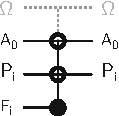
\includegraphics[width=2.5cm]{graphics/development/editing_hivent_data/edit_to_hivent_operations/CHB_to_SEC+INC_omega}
  } \\
  &
  $n_f$ &
  $1+n_p$ &
  $0$ &
  \pbox{6.0cm}{
    ~\\
    \texttt{SEC} of $T_\Omega$ from $\Omega$,
    \texttt{INC} of $T_\Omega$ into $A_0$ \\
    \texttt{SEC} of $T_p$ from $A_p$,
    \texttt{INC} of $T_p$ into $B_1$ \\
    \texttt{INC} of $A_f$ into $B_1$ \\
    \texttt{SEC} of $T_w$ from $B_1$,
    \texttt{INC} of $T_w$ into $\Omega$
  } &
  \\

  \midrule
  \multirow{7}{*}{\texttt{CHB} (2)} &
  \multicolumn{4}{p{10cm}}{
    Two existing Areas $A_1$ and $A_2$ are selected and their common border changes. This results in a symmetrical change of territories, made up by two sets of territories: $T_2$ that previously belonged to $A_1$ and is now part of $A_2$ and $T_1$ for which the opposite is true. $T_2$ is seceded by $A_1$ and incorporated into $A_2$, the opposite happenes to $T_1$.
  } &
  \multirow{7}{*}{
    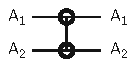
\includegraphics[width=2.5cm]{graphics/development/editing_hivent_data/edit_to_hivent_operations/CHB_to_SEC+INC}
  } \\
  &
  $0$ &
  $2$ &
  $0$ &
  \pbox{6.0cm}{
    ~\\
    \texttt{SEC} of $T_2$ from $A_1$,
    \texttt{INC} of $T_2$ into $A_2$ \\
    \texttt{SEC} of $T_1$ from $A_2$,
    \texttt{INC} of $T_1$ into $A_1$
  } &
  \\

  %%% RENAME %%%

  \midrule
  \multirow{3}{*}{\texttt{REN} (1)} &
  \multicolumn{4}{p{10cm}}{
    One Area $A_1$ is selected and both its short and formal name is changed. Therefore, a new Area $B_1$ is created as a direct successor of $A_1$. This is a special case of a unification with only one Area.
  } &
  \multirow{3}{*}{
    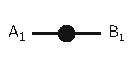
\includegraphics[width=2.5cm]{graphics/development/editing_hivent_data/edit_to_hivent_operations/REN_to_UNI}
  } \\
  &
  $1$ &
  $0$ &
  $1$ &
  \pbox{6.0cm}{
    \texttt{UNI} of $A_1$ to $B_1$
  } &
  \\

  \midrule
  \multirow{3}{*}{\texttt{REN} (2)} &
  \multicolumn{4}{p{10cm}}{
    One Area $A_1$ is selected and receives a new short name, but the formal name and therefore the identity is preserved. $A_1$ is updated.
  } &
  \multirow{3}{*}{
    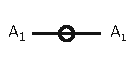
\includegraphics[width=2.5cm]{graphics/development/editing_hivent_data/edit_to_hivent_operations/REN_to_NCH}
  } \\
  &
  $0$ &
  $1$ &
  $0$ &
  \pbox{6.0cm}{
    \texttt{NCH} of $A_1$
  } &
  \\

  %%% CEASE %%%

  \midrule
  \multirow{2}{*}{\texttt{CES} (1)} &
  \multicolumn{4}{p{10cm}}{
    One Area $A_1$ is selected and ceases by incorporating into the universe.
  } &
  \multirow{2}{*}{
    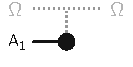
\includegraphics[width=2.5cm]{graphics/development/editing_hivent_data/edit_to_hivent_operations/CES_to_INC}
  } \\
  &
  $1$ &
  $0$ &
  $0$ &
  \pbox{6.0cm}{
    \texttt{INC} of $A_1$ into $\Omega$
  } &
  \\

  \bottomrule
\caption{Translation from Edit Operations to Hivent Operations}
\end{longtable}
\label{tab:editoperations_to_hg_operations}
\end{center}
\footnotetext{multiple Hivent Operations in one row happen exactly at the same time point, so they are combined}


% subsection edit_workflow (end)

% ------------------------------------------------------------------------------
\subsection{Retrospective Updates} % (fold)
\label{sub:retrospective_updates}

A straightforward use case of the Hivent Model is to change the current state of the system with a new Hivent Operation into the future. Givent the initial start point $t_0$, a current time point $t_{now} > t_0$ and a set of consecutively added Hivent Operations at $\forall t_i: t_0 \leq t_i < t_{now}$. The accumulation of all changes make up the current state of the system at $t_{now}$. To change this current state, a new Hivent Operation can be inserted at $t_{now}$ into the future. This state is valid until the next change is inserted.

For historical research that use case alone is not sufficient, because the current state of the map at $t_{now}$ (2016) is known to a large degree. The problem is to describe states and changes in the past. Therefore the systems needs to support entering Hivent Operations in between other existing operations.


% - - - - - - - - - - - - - - - - - - - - - - - - - - - - - - - - - - - - - - -
\paragraph{Integrity} % (fold)
\label{par:integrity}

Each Hivent Operation that is not entered to the end of the timeline must maintain the semantic, spatial and thematic integrity of the data, i.e. the changes to Areas, their territories and names must still work. The simple example in figure \ref{fig:update_conflict_example} shows the problem: Given time point $t_1$ with two Areas $A$ and $B$ and an \texttt{UNI} Hivent Operation at $t_2$ unifying $A$ and $B$ to $C$. If in retrospective a new Hivent Operation is inserted at $t_r: t_1 < t_r < t_2$ that cedes a part of of $A$ to a new Area $X$, the operation at $t_2$ is not consistent anymore, because the old territory of $A$ is not the same. It is not simple to say how the remaining territory $?$ should be treated.

\begin{figure}[H]
  \vspace{1em}
  \centering
  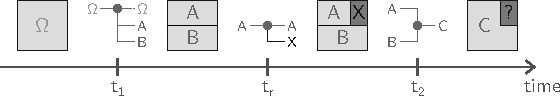
\includegraphics[width=0.8\textwidth]{graphics/development/editing_hivent_data/retrospective_updates/example}
  \caption{Example for a simple conflict due to a retrospective update}
  \label{fig:update_conflict_example}
\end{figure}

% paragraph integrity (end)

% - - - - - - - - - - - - - - - - - - - - - - - - - - - - - - - - - - - - - - -
\paragraph{Conflicts} % (fold)
\label{par:conflicts}

The way the Hivent Model works is comparable to a version control system like \emph{Git}
\footnote{
  \emph{Git},
  - -everything-is-local,
  \url{https://git-scm.com/},
  last access: 29.05.2016
}
There are different kinds of conflicts that can occur on retrospective updates. In the Hivent Model, they are classified regarding their resolvability:

\begin{compactenum}
  \item[A)] The conflict can be resolved \emph{\textbf{a}utomatically} without the interference of the user.
  \item[S)] The conflict requires the user to choose between two alternatives (\emph{\textbf{s}emi-automatic} resolution).
  \item[M)] The conflict is complex and the user needs to resolve it \emph{\textbf{m}anually}.
\end{compactenum}

The remaining part of this section examines all possible cases of conflicts and their resolveability. Each inserted Hivent Operation transforms a set of old Areas $A = [A_i]$ to a set of new Areas $B = [B_i]$ or updates an update Area $A_0$ or both. Each consecutive Hivent Operation that manipulates $A_0, A_i \in A$ or $B_i \in B$ has to be checked regarding three aspects of integrity:

\begin{compactenum}
  \item semantic: Does $A_0$ and $\forall A_i \in A$ still exist? If not, can it easily be replaced by another Area?
  \item spatial: Is the territory of $A_0$ and $\forall A_i \in A$ still the same? If not, can it easily by updated?
  \item thematic: Is the name of $A_0$ and $\forall A_i \in A$ still the same? If not, can it easily be updated?
\end{compactenum}

All cases can be simulated in the following simple scenario: Given the system with only two states: an initial state at $t_1$ at which only three spatial entities are on the map ($A_1, A_2, A_3$) and an Hivent Operation at $t_2$ that manipulates some of these Areas with one of the five possible operations. This is called the original Hivent Operation ($H_o$). Now, a retrospective update $H_r$ is inserted in between the two states ($t_r: t_1 < t_r < t_2$). $H_r$ manipulates the same set of Areas with an Hivent Operations. The question is: What happens regarding the semantic, spatial and thematic integrity of $H_o$? Is there a conflict and if so, hw can it be resolved? There are 25 possible cases, because for both $H_o$ and $H_r$ there are five possible Hivent Operations.

% paragraph conflicts (end)

% - - - - - - - - - - - - - - - - - - - - - - - - - - - - - - - - - - - - - - -
\paragraph{Retrospective Name Change} % (fold)
\label{par:retrospective_name_change}

The first five cases are straightforward: Given \texttt{NCH} is inserted in retrospective ($H_r$) to change the name of $A_1$ from $X$ to $Y$. This has no effect on the identity or territory of $A_1$. Therefore the system only needs to check for thematic integrity of $H_o$. If that operation is an \texttt{INC} or \texttt{SEC}, which both only change the territory of $A_1$, it is not conflicting. If $H_o$ is a \texttt{UNI} or \texttt{SEP}, then there is a conflict: $A_1$ is an old Area of the operation, but the name associated to $A_1$ is still $X$. This is not consistent, because $H_r$ just changed the name to $Y$ . This conflict can be resolved automatically by updating the name in the old Area from $X$ to $Y$. The same is true if $H_o$ is a \texttt{NCH} operation: $A_1$ is the update Area and the old name has to be updated from $X$ to $Y$. To summarize what the system has to do if a \texttt{NCH} on $A_1$ is inserted in retrospective: find the next \texttt{UNI}, \texttt{SEP} or \texttt{NCH} operation that manipulates $A_1$ and update its old name.

% paragraph retrospective_name_change (end)

% - - - - - - - - - - - - - - - - - - - - - - - - - - - - - - - - - - - - - - -
\paragraph{Retrospective Incorporation} % (fold)
\label{par:retrospective_incorporation}

An \texttt{INC} ceases a set of old Areas and changes the territory of one Area. In this scenario, $H_r$ incorporates $A_2$ into $A_1$. The question is what kind of conflicts can occur to the spatial integrity of $H_o$? If $H_o$ is  a \texttt{NCH}, there is no conflict, because $H_o$ changes the territory of $A_1$ and \texttt{NCH} the name.

\begin{figure}[ht]
\vspace{1em}
  \centering
  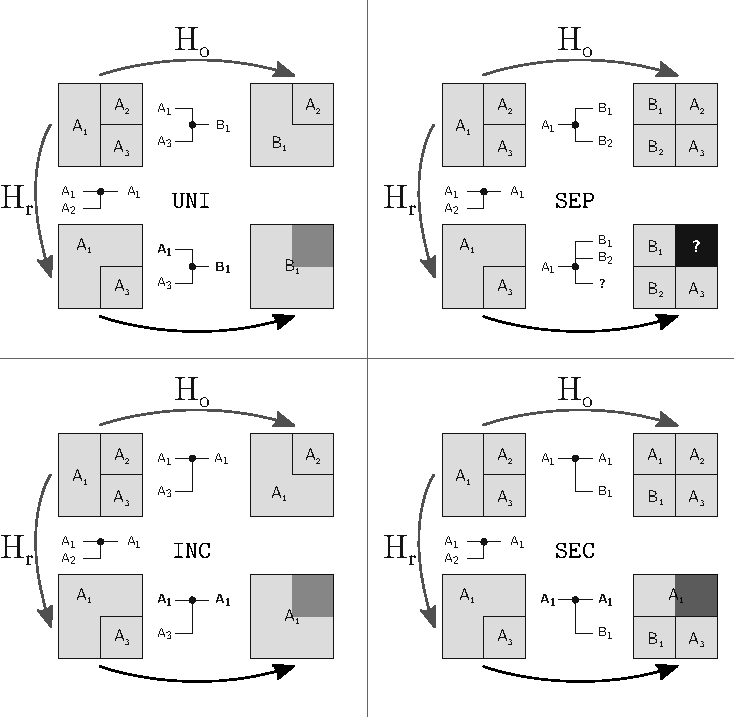
\includegraphics[width=0.8\textwidth]{graphics/development/editing_hivent_data/retrospective_updates/INC}
  \caption{Conflicts after a retrospective incorporation}
  \label{fig:update_conflict_INC}
\end{figure}

Figure \ref{fig:update_conflict_INC} shows the conflicts that occur in the remaining four possiblities of $H_o$. In the case of an original \texttt{UNI} operation, it can still be performed with the same Areas, because $H_r$ did not change the identity of $A_1$. However, the territory of $A_1$ has been enlarged. This new territory has to be taken into account for $H_o$: To maintain spatial integrity, the system has to update the territory of incoming $A_1$. However, the territory of $B_1$ has to be updated as well, because it is enlarged in the same way as $A_1$. This requires a recursive update into the future: the next Hivent Operation dealing with $B_1$ needs to take into account that the territory has changed. This case can be treated as if $H_o$ would be $H_r$ with an \texttt{INC} operation. The system has to repeat this process until all conflicts are solved. The same is true if $H_o$ is an \texttt{INC} operation: The system needs to update the old and the new territory of $A_1$ in $H_o$ and recursively update the territory of $A_1$ into the future.

If $H_o$ is a \texttt{SEP} operation, there is a major conflict: originally, $A_1$ splitted into $B_1$ and $B_2$. Due to $H_r$, the territory of $A_1$ is larger. $H_o$ can still separate $B_1$ and $B_2$ from $A_1$ the same way as before, but it is unclear what should happen to the remaning territory of $A_1$ that has just been enlarged. This conflict has to be resolved manually, because the system can not derive a decision from any existing information. The remaining part could become $\Omega$, it could be incorporated into $B_1$ or $B_2$ or stay $A_1$. However, the user has to decide it. In case of an original \texttt{SEC}, the situation is slightly different: $H_1$ still exists like before, just with a larger territory. $H_o$ can secede $B_1$ like originally, but the system needs to update the old and new territory of $A_1$ in this operation and recursively into the future.

The foregoing investigation relates only to $A_1$ but not to $A_2$ that has been incorporated into $H_r$. From the perspective of $A_2$, this change can be seen as a \texttt{UNI}, because its identity ceases and together with its territory it completely merges into $A_1$. Therefore this is treated like a retrospective unification examined later in this section.

% paragraph retrospective_incorporation (end)

% - - - - - - - - - - - - - - - - - - - - - - - - - - - - - - - - - - - - - - -
\paragraph{Retrospective Secession} % (fold)
\label{par:retrospective_secession}

Retrospective secessions are comparable to incorporations: The identity and the name of $A_1$ does not change -- but parts of its territory ceases to a new Area $B_1$. This section examines how the system has to treat $B_1$ and the smaller territory of $A_1$ in the original operation $H_o$. Exactly like for retrospective incorporation, there is no conflict if $H_o$ is a \texttt{NCH}.

\begin{figure}[ht]
\vspace{1em}
  \centering
  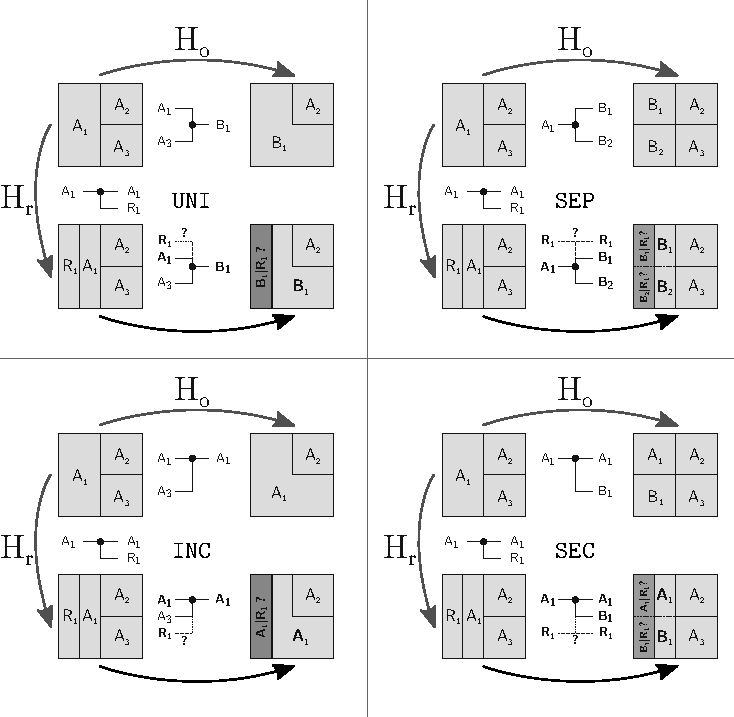
\includegraphics[width=0.8\textwidth]{graphics/development/editing_hivent_data/retrospective_updates/SEC}
  \caption{Conflicts after a retrospective secession}
  \label{fig:update_conflict_SEC}
\end{figure}

The other four cases are visualized in figure \ref{fig:update_conflict_SEC}. For an original \texttt{UNI}, there is a conflict: Originally, $A_1$ and $A_3$ unified to $B_1$. Although $H_r$ cedes parts of the territory of $A_1$ to $R_1$, $H_o$ can still merge it with $A_3$. The question is what happens to the remaining territory of $R_1$? There are two options:
\begin{compactenum}
  \item
  \emph{priority to $H_r$}:
  $R_1$ stays an own Area and is not affected by $H_o$.
  \item
  \emph{priority to $H_o$}:
  $H_o$ unifies $R_1$ to $B_1$ as well.
\end{compactenum}
For the system it is hard to decide this, because it is unclear what the intention of the user is when creating $R_1$ in $H_r$: Should the newly created Area be there for longer or is the territory of the unitied Area $A_3$ more important? In order for the system to not behave unexpectedly, it will ask the user which choice he or she prefers. In case of the first choice, the territory of $R_1$ has to be subtracted from the territory of the new Area $B_1$ in $H_o$. This update is again recursive, because the next Hivent Operation dealing with $B_1$ needs to operate on the correct territory as well. In the second case, $R_1$ simply has to be added to the old Areas of the \texttt{UNI} operation in $H_o$. No further recursive update is necessary. The same behavior is true if $H_o$ is an \texttt{INC}. The user has to decide if he or she wants to incorporate $R_1$ into $A_1$ or keep it as a separate Area. In the latter case, the system needs to update the new territory of $A_1$ in $H_o$.

For an original \texttt{SEP}, the situation is comparable: Originally, $A_1$ splits into $B_1$ and $B_2$, but after the restrospective secession of a part of $A_1$ to $R_1$, the territory of $R_1$ is conflicting with $B_1$ and $B_2$ in $H_o$. An important observation is that each part of $R_1$ would be part of either $B_1$ or $B_2$. There is no empty land, since both $R_1$ and $B_1+B_2$ seceded from the same territory of $A_1$. Just like the other two cases above, the system will give the user for both conflicting territories the choice if either $R_1$ should stay an Area or if $B_1$ respectively $B_2$ should incorporate $R_1$ into their territory. In the first case, the territory of $R_1$ has to be subtracted both from the incoming $A_1$ and recursively from the outgoing territory $B_1$ respectively $B_2$. The latter case needs at least one additional Hivent Operation: the part of $R_1$ that shall be part of $B_1$ respectively $B_2$ needs to be seceded from $R_1$ and the same time incorporated into $A_1$ which then again in the same moment is separated into $B_1$ and $B_2$ ($H_o$ = \texttt{SEC+INC+SEP}). If whole $R_1$ ceases in the operation, then it is incorporated into $A_1$ completely, so it is only a \texttt{INC+SEP} at $H_o$. The case of an orginal \texttt{SEC} the system behaves in exactly the same way, just with an update of the territory of $A_1$ and $B_1$ instead of $B_1$ and $B_2$.

To summarize, the main difference between retrospective incorporation and secession is that in the latter case, the user needs to choose between two predefined options. For incorporations, this is seen as unnecessary, because the conflicting territory of $A_2$ has not been manipulated by $H_o$, so it can not be seen as a concious decision of the user to keep this Area.

% paragraph retrospective_secession (end)

% - - - - - - - - - - - - - - - - - - - - - - - - - - - - - - - - - - - - - - -
\paragraph{Retrospective Unification} % (fold)
\label{par:retrospective_unification}

If a \texttt{UNI} is inserted in retrospective, the semantic integrity of $H_o$ is threatened, because in contrast to a \texttt{INC} all incoming Areas cease and unify to one completely new Area, in this example $R_1$. For each Area $A_i \in A$ that was unified in $H_r$ the system needs to find the next Hivent Operation $H_o$ manipulating $A_i$ and update it accordingly. In this example, $A_1$ is examined in place of each $A_i \in A$. If $H_o$ is a \texttt{NCH}, there is a conflict: the name of $A_1$ can obviously not be updated anymore, because $A$ does not exist aynmore. The only way to resolve this conflict is to automatically delete the \texttt{NCH} operation. All the other four cases behave regarding spatial integrity in exactly the same way as for a retrospective incorporation -- with the only difference that the Area $A_1$ is replaced by $R_1$ as an incoming Area in the operation. In all four cases, the territory has to be updated in the same way as for retrospective incorporation and the same conflict occurs for the original \texttt{SEP} operation.

\begin{figure}[ht]
\vspace{1em}
  \centering
  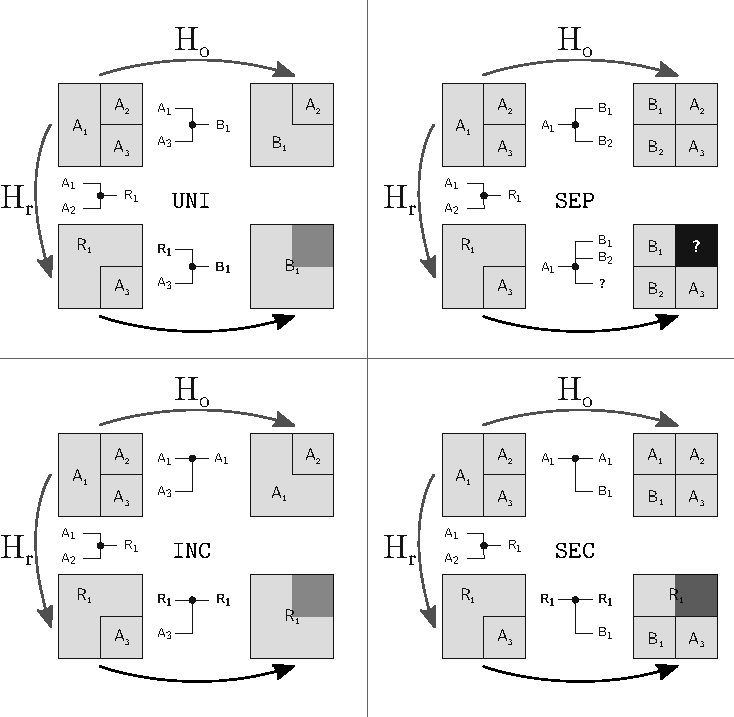
\includegraphics[width=0.8\textwidth]{graphics/development/editing_hivent_data/retrospective_updates/UNI}
  \caption{Conflicts after a retrospective unification}
  \label{fig:update_conflict_UNI}
\end{figure}

% paragraph retrospective_unification (end)

% - - - - - - - - - - - - - - - - - - - - - - - - - - - - - - - - - - - - - - -
\paragraph{Retrospective Separation} % (fold)
\label{par:retrospective_separation}

In contrast to the previous example, retrospective separations behave slightly different from secessions. $H_o$ has to be checked both for spatial and semantic integrity, since $A_1$ ceased in $H_r$ to a set of new Areas $R_i$. In this scenario, $R_1$ and $R_2$ stay in place for $\forall r_i \in R$. If $H_o$ is a \texttt{NCH}, the operation has to be automatically deleted, because $A_1$ does not exist anymore. Figure \ref{par:retrospective_separation} shows the conflicts that arise for the remaining four cases.

\begin{figure}[ht]
\vspace{1em}
  \centering
  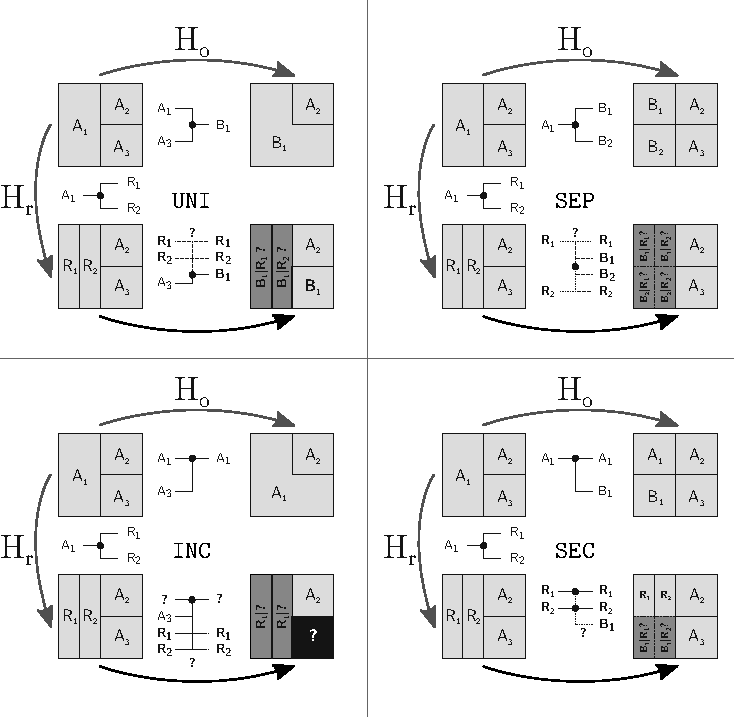
\includegraphics[width=0.8\textwidth]{graphics/development/editing_hivent_data/retrospective_updates/SEP}
  \caption{Conflicts after a retrospective separation}
  \label{fig:update_conflict_SEP}
\end{figure}

In case $H_o$ is a \texttt{UNI}, the arising conflict can be solved semi-automatically: originally, $B_1$ was created by unifying $A_1$ and $A_3$. $A_1$ just got separated into $R_1$ and $R_2$ by $H_r$, so the system can not know if $R_1$, $R_2$ or $B_1$ is preferred at $H_o$. In any case, the system needs to remove $A_1$ form the old Areas in the \texttt{UNI} operation. For each created Area in $H_r$ -- in this case only $R_1$ and $R_2$ -- the system asks the user if he or she prefers $R_i$ or $B_1$. If $R_1$ is preferred, then its territory has to be recursively subtracted from from the outgoing Area $B_1$ in the \texttt{UNI} operation at $H_o$. Else $R_i$ is added to the old Areas of $H_o$. If $R_i$ is preferred every time, the remaining \texttt{UNI} operation only transforms $A_3$ to $B_1$.

If $H_o$ is an \texttt{INC}, the situation is more complex: The Area $A_1$ in which $A_3$ should be incorporated into does not exist anymore. Moreover, it is replaced by a set of new Areas $R_i$ and it is not straightforward to see where $A_3$ should be incorporated into -- it is only clear that $A_3$ will cease in this operation. Since there is no information about what should be there instead, this conflict has be solved manually. The situation is even more complicated, because on the one hand, in $H_o$ the user intentionally incorporated $A_3$ into $A_1$ which means there is an obvious intention to keep $A_1$. On the other hand, he or she separated $A_1$ in $H_r$ to two new Areas $R_1$ and $R_2$, so also they can be seen as intenionally created. To avoid an unexpected behavior of the system, the best approach is give him or her the choice to keep $R_1$ and $R_2$, but in case of denial let the user resolve the whole conflict manually.

The case of an original \texttt{SEP} is likewise complex: $A_1$ does not exist anymore to be separated -- instead there are two sets of Areas that can be seen as reasonable to be the outcome of the operation: On the one hand the Areas $B_i \in B$ created in $H_o$ and on the other hand $R_j \in R$ created in $H_r$. Since it is impossible for the system to know which Areas to prefer, the user should decide for each possible combination $i \times j$ which Area it should be. If $R_j$ is preferred, then its territory has to be recursively subtracted from each $B_i$ that intersects with $R_j$. Else the territory of $R_j$ intersecting with $B_i$ has to secede from $R_j$ and be incorporated into $B_i$ with a combination of \texttt{SEC+INC} at $H_o$. The \texttt{SEP} operation itself it not necessary anymore, because there is not one simple old Area anymore.

The last case to examine is the influence of a retrospective \texttt{SEP} on an original \texttt{SEC}. Originally, $\forall B_i \in B$ would secede from $A_1$, which has just been separated into $\forall R_j \in R$ in $H_r$. The part of the territory of each $R_j \in R$ not covered by any $B_i \in B$ will certainly stay $R_j$, because there is no other reasonable alternative. The conflict is at the overlapping territory between $B_i$ and $R_j$. Just like for the previous example, the user has to resolve these conflicts semi-automatically by choosing either $B_i$ or $R_j$ for each possible alternative. If $B_i$ is preferred, it is seceded from the related $R_j$ at $H_o$. If $R_j$ is preferred, its territory has be recursively subtracted from the related $B_i$.

% paragraph retrospective_separation (end)

% - - - - - - - - - - - - - - - - - - - - - - - - - - - - - - - - - - - - - - -
\vspace{1em}
\begin{table}[ht]
\begin{center}
\begin{tabular}{p{0.1cm} p{0.1cm} p{0.3cm} cx{2.0cm} cx{2.0cm} cx{2.0cm} cx{2.0cm} cx{2.0cm} cx{2.0cm}}
  \toprule
  & & & & \multicolumn{5}{c}{original Hivent Operation $H_o$} \\
  & & & & \texttt{UNI} & \texttt{SEP} & \texttt{INC} & \texttt{SEC} & \texttt{NCH} \\
  \midrule
    \multirow{5}{*}{\rot{retrospective}}
  & \multirow{5}{*}{\rot{operation $H_r$}}
    & & \texttt{UNI} & A & \textbf{M} & A & A & A \\
  & & & \texttt{SEP} & S(A$|$A) & S(A$|$A) & \textbf{M} & S(A$|$A) & A \\
  & & & \texttt{INC} & A & \textbf{M} & A & A & X \\
  & & & \texttt{SEC} & S(A$|$A) & S(A$|$A) & S(A$|$A) & S(A$|$A) & X \\
  & & & \texttt{NCH} & A & A & X & X & A \\
  \bottomrule
\end{tabular}
\caption{All possible conflicts on retrospective updates regarding their resolvability}
\small{X = no conflict, A = automatic, S = semi-automatic, \textbf{M} = manual resolution \\[-0.1em]
For semi-automatic resolution, the resolveability of the two options is stated like S(\nth{1}$|$\nth{2})}
\label{tab:conflicts_retrospective_updates}
\end{center}
\end{table}

All possible cases and their resolvability are visualized in the $5 \times 5$ matrix in figure \ref{tab:conflicts_retrospective_updates}. It became clear in the extensive examnination of the conflicting cases that inserting a retrospective update into a spatio-temporal system is not straightforward at all. Especially if a separation or secession is added somewhere not to the end of the timeline, in almost all cases the user has to decide between two alternatives. In three cases there is even a manual resolution necessary. A lot of cases also require recursive updates, meaning the retrospective update can lead to a potentially high number of semi-automatic or even manual resolutions by the user, which an potentially be frustrating. On top of that the examination completely disregarded the situation of combined cases, e.g. if the original operation is a combination of \texttt{SEC+INC} resulting from a user-defined border change (\texttt{BCH}) between two Areas. This might become even more complex. In summary, the Hivent Model needs to be checked for potential adaptions that might simplify retrospective updates and make the data handling less frustrating.

% subsection retrospective_updates (end)

% ------------------------------------------------------------------------------
\subsection{Backward Operations} % (fold)
\label{sub:backward_operations}

From a relative time point $t_i$ there are two historical directions: forward into the future with a predefined end at the current time point $t_{now}$ and backward into the past until the predefined start point of the system $t_0$. Everything until now was focused on \texttt{forward operations} that change the current state of the system at the set time point $t_i$ into the future, either until another operation changes it again or until $t_{now}$.

As it has been argued in the previous section \ref{sub:retrospective_updates} for retrospective updates, only forward operations to the end of the timeline are not sufficient for historical research. For an historian to edit a state in the past, a \texttt{backward operation} might be useful: A Hivent Operation is inserted at time point $t_i$, but into the past: $ t_0 < t_i < t_{now}$. As an example: Given the initial state 10.06.2016 with present-day Germany created on 03.10.1990 on the map. The user wants to enter the German Reunification. The HGIS must support separating Germany into East and West, but indicating that this was the state \emph{before} 1990 and the original state was \emph{after} this date. This is complicated, because the conceptual, data and computational model have to adapt to this requirement.

The Hivent Operations themselves allow to be executed the other way, because each of them has an inverse operation: A \texttt{UNI} can be inverted with a \texttt{SEP} and a \texttt{INC} with a \texttt{SEC} operation. \texttt{NCH} can be inverted with itself by swapping the old and new name.

One problem is the conceptual model: The user interface has to provide a visual clue that inverting the direction of an operation is possible. Additionally, if an Hivent Operation is inserted backwards, another problems comes into play: all new Areas of the operation would now be active from $t_i$ on backwards into the \emph{past}. Each Area that is created in a backward operation has to be provided with another operation that ceases it in backward direction or creates it in forward direction, otherwise the Area would be active all the back to $t_0$. This is probably not desirable.

%TODO: graphic?

% subsection backward_operations (end)

% section editing_hivent_data (end)
%!TEX root = ../masters_thesis.tex

\section{User Interface Design Process} % (fold)
\label{sec:user_interface_design_process}

The Hivent Model presented in the previous section serves as the data model for HistoGlobe, the application in which the work of this thesis is implemented. Developing the system bottom-up from the data model to the interface might not lead to usable system. Human Centered Design promotes a top-down process from the user via the interface into the core of the application. This section illustrates the iterative design process for this thesis seen in figure \ref{fig:hcd}. The two main use cases for HistoGlobe that are focused in this thesis are:

\begin{compactenum}
  \item \textbf{Understanding} the history of countries.
  \item \textbf{Editing} the spatio-temporal evolution of countries with historical changes.
\end{compactenum}

For both use cases a visualization and interaction was designed. The interviews with humanity researchers confirmed that the combination of a map and a timeline are a very appropriate and intuitive way to interactively visualize the history of countries. Thefore, the main concept of HistoGlobe introduced in section \ref{sec:histoglobe} does not need to be changed. However, two necessary extension modules have emerged: The \emph{HistoGraph} introduced in section \ref{sub:histograph} visualizes the history of countries on a graph. Next to the normal browsing mode, the \emph{Edit Mode} is proposed in section \ref{sub:edit_mode}. It uses the six Edit Operations to introduce historical changes to the current state on the map. The gradual process from the inital idea to the final user interface implemented in HistoGlobe is illustrated in the last section-

The user interface of HistoGlobe has two modi: The browsing mode to view the evolution of countries on a map with a timeline and the \emph{Edit Mode} to introduce historical changes to Areas. This mode is proposed in this section. The Human Centered Design process produced an interface that allows to intuitively edit Hivents, Areas and historical changes directly in HistoGlobe, without the need to write data into tables or forms.

The previous sections introduced the concepts of the HistoGraph and the Edit Mode. This section illustrates the Human Centered Design process integrating both concepts into the existing user interface of HistoGlobe. In each phase, interviews with students and employees of Scholar's Lab at University of Virginia were conducted to determine what works well and what has to be improved.

% - - - - - - - - - - - - - - - - - - - - - - - - - - - - - - - - - - - - - - -
\subsection{Initial interviews} % (fold)
\label{sub:initial_interviews}

The first phase, four researchers were asked about their opinions on the idea of HistoGlobe, potential use cases and the concept of the Edit Mode. The idea proved popular, especially for students and teachers in school, historically interested people in general and also for scholars in digital humanities. All researchers agreed that the key to successful Edit Mode is usability, because editing data in time and space is a challenging task. A main concern is uncertainty in historical research: Almost all sorts of information -- temporal, spatial and attribute -- are potentially uncertain. A good user interface for researchers therefore has to support uploading historical sources and indicating uncertainty. The Edit Operations from section \ref{sub:edit_operations} resulted from the initial interviews.

% subsection initial_interviews (end)


% - - - - - - - - - - - - - - - - - - - - - - - - - - - - - - - - - - - - - - -
\subsection{Paper Prototype} % (fold)
\label{sub:paper_prototype}

From the results of the inital interview, the first interface concept for the Edit Mode was developed and transformed into a paper prototype. It is an interface out of paper that is very fast to create and allows to identify flaws in the concept early in the design process. In this process, two paper prototype iterations were created. Both iteration took about three full work days: one day to create the conceptualize and create prototype, half a day to conduct the study with three people, and one and a half days to analyze the results and rethink the concept.

\begin{figure}[H]
\centering
\begin{subfigure}{.5\textwidth}
  \centering
  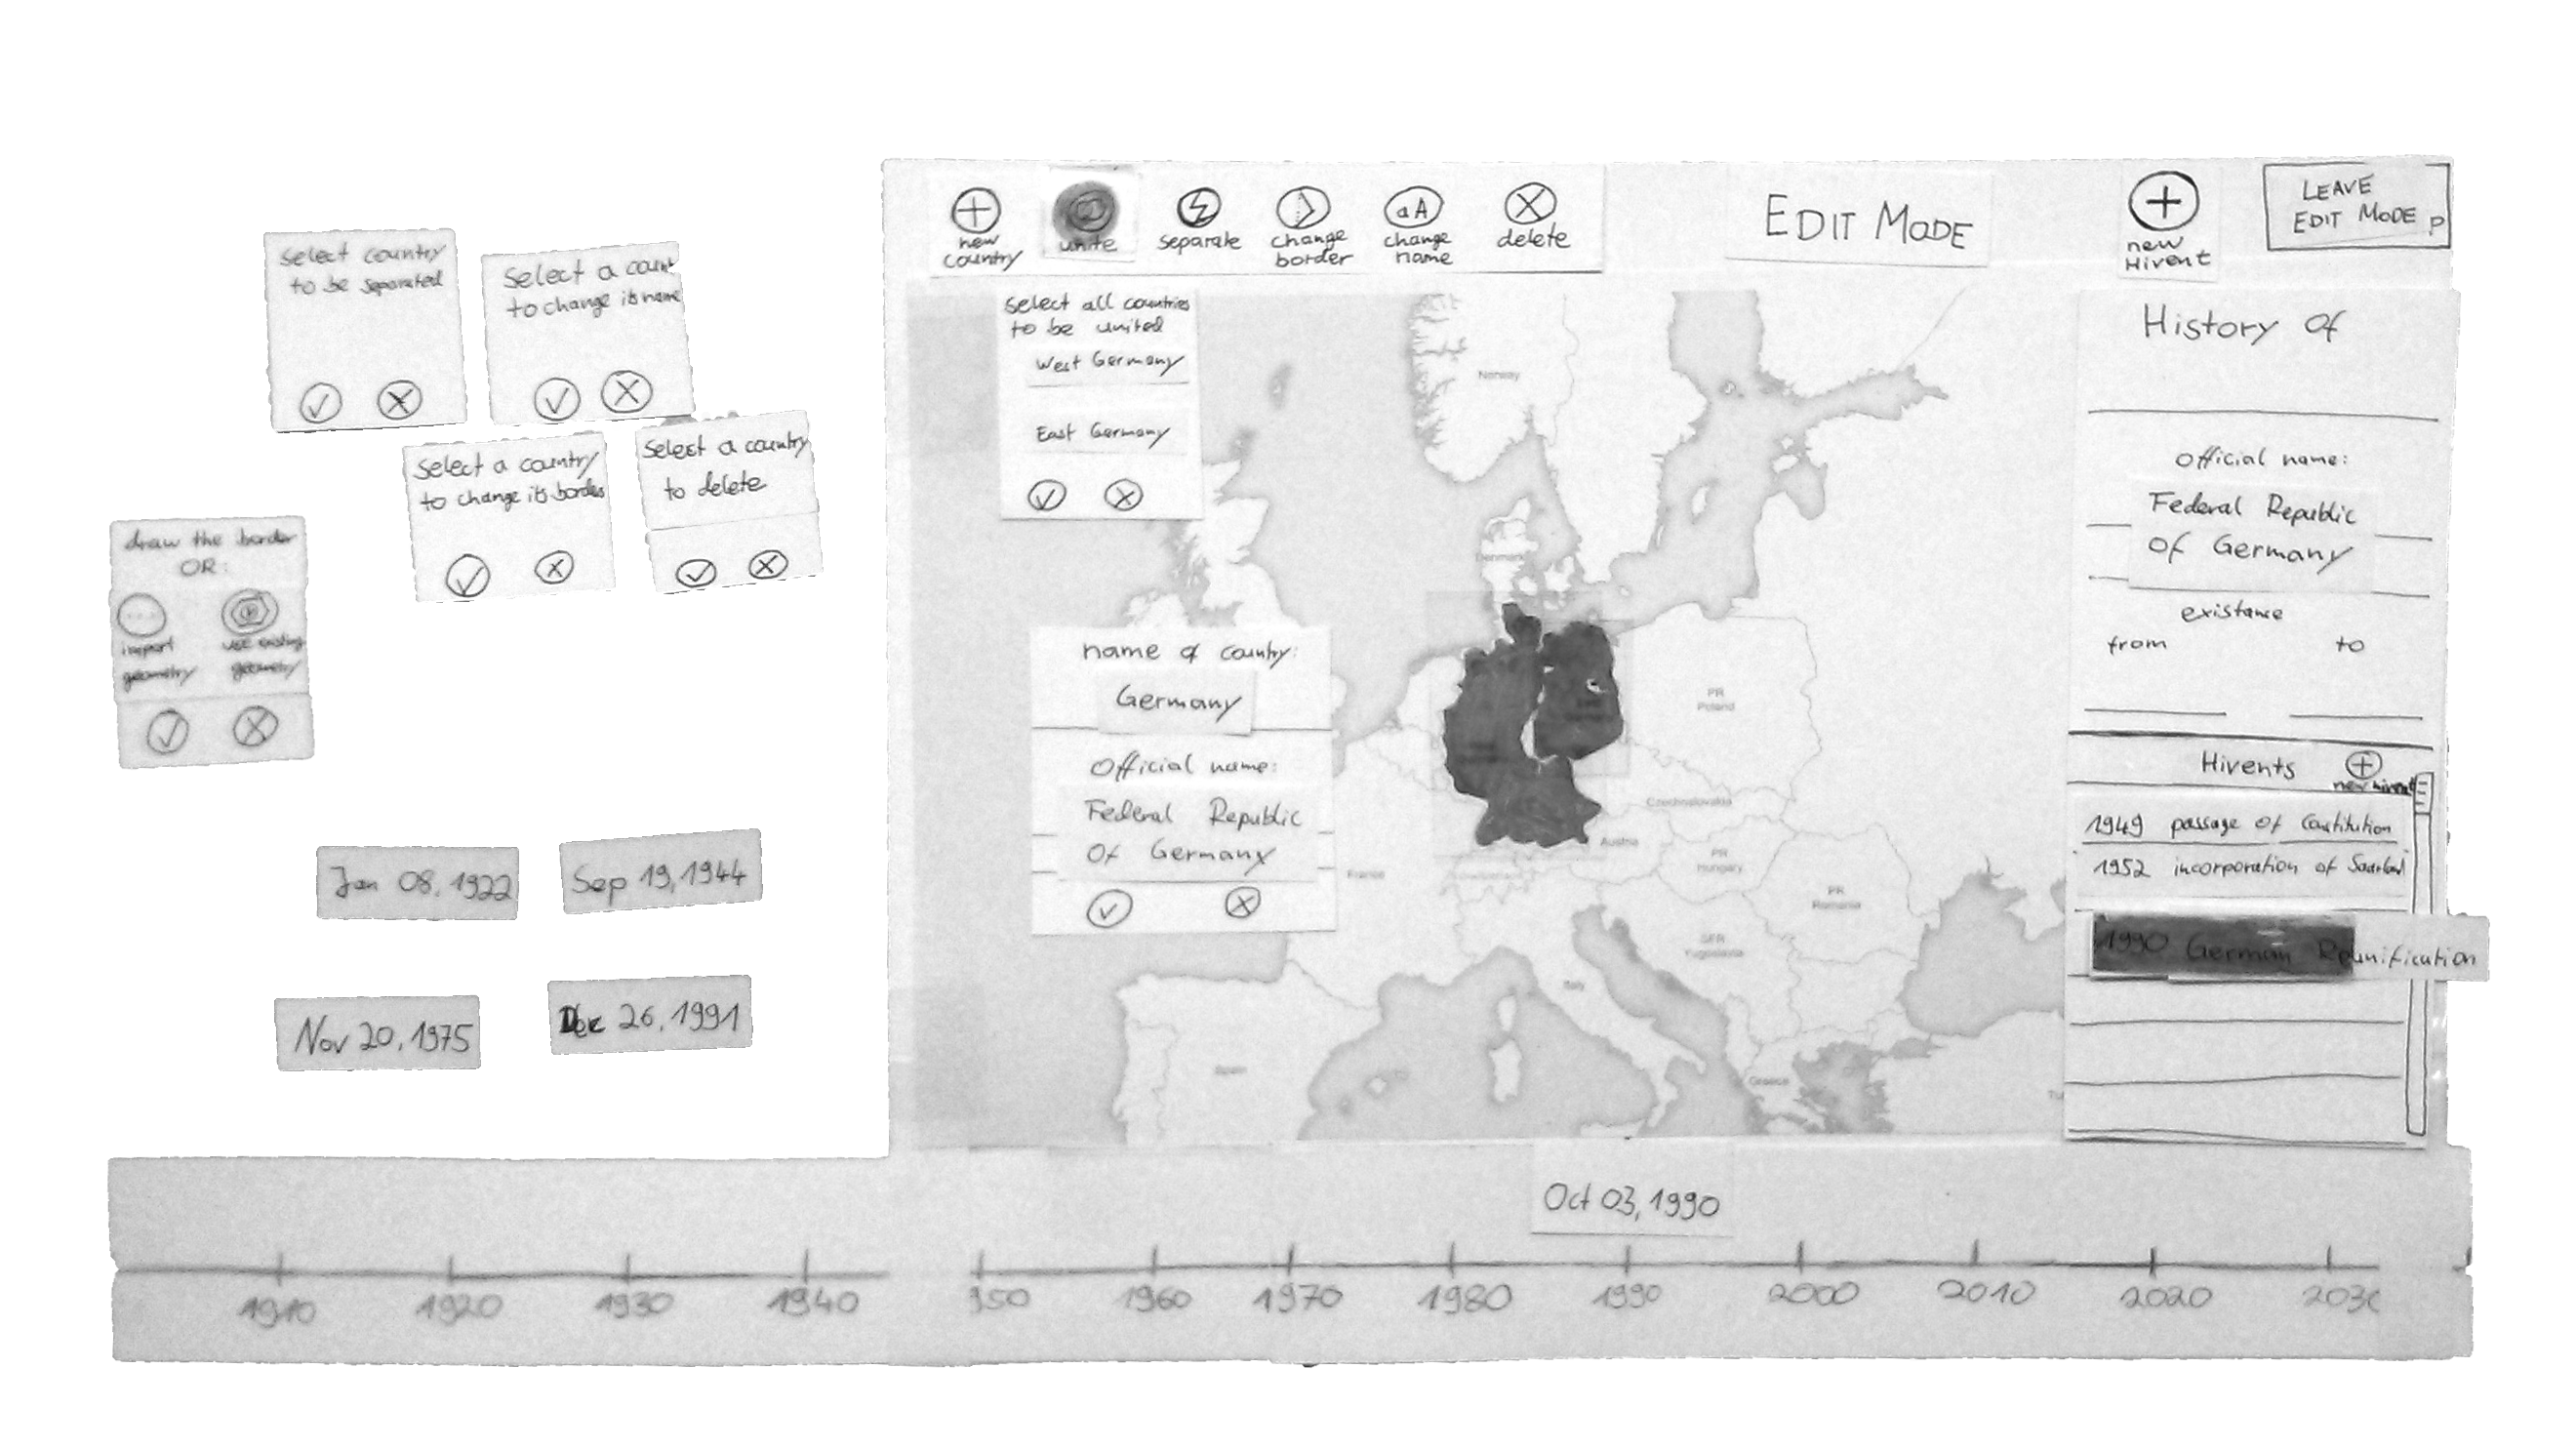
\includegraphics[width=225px]{graphics/development/design_process/paper_prototype_1.png}
\end{subfigure}%
\begin{subfigure}{.5\textwidth}
  \centering
  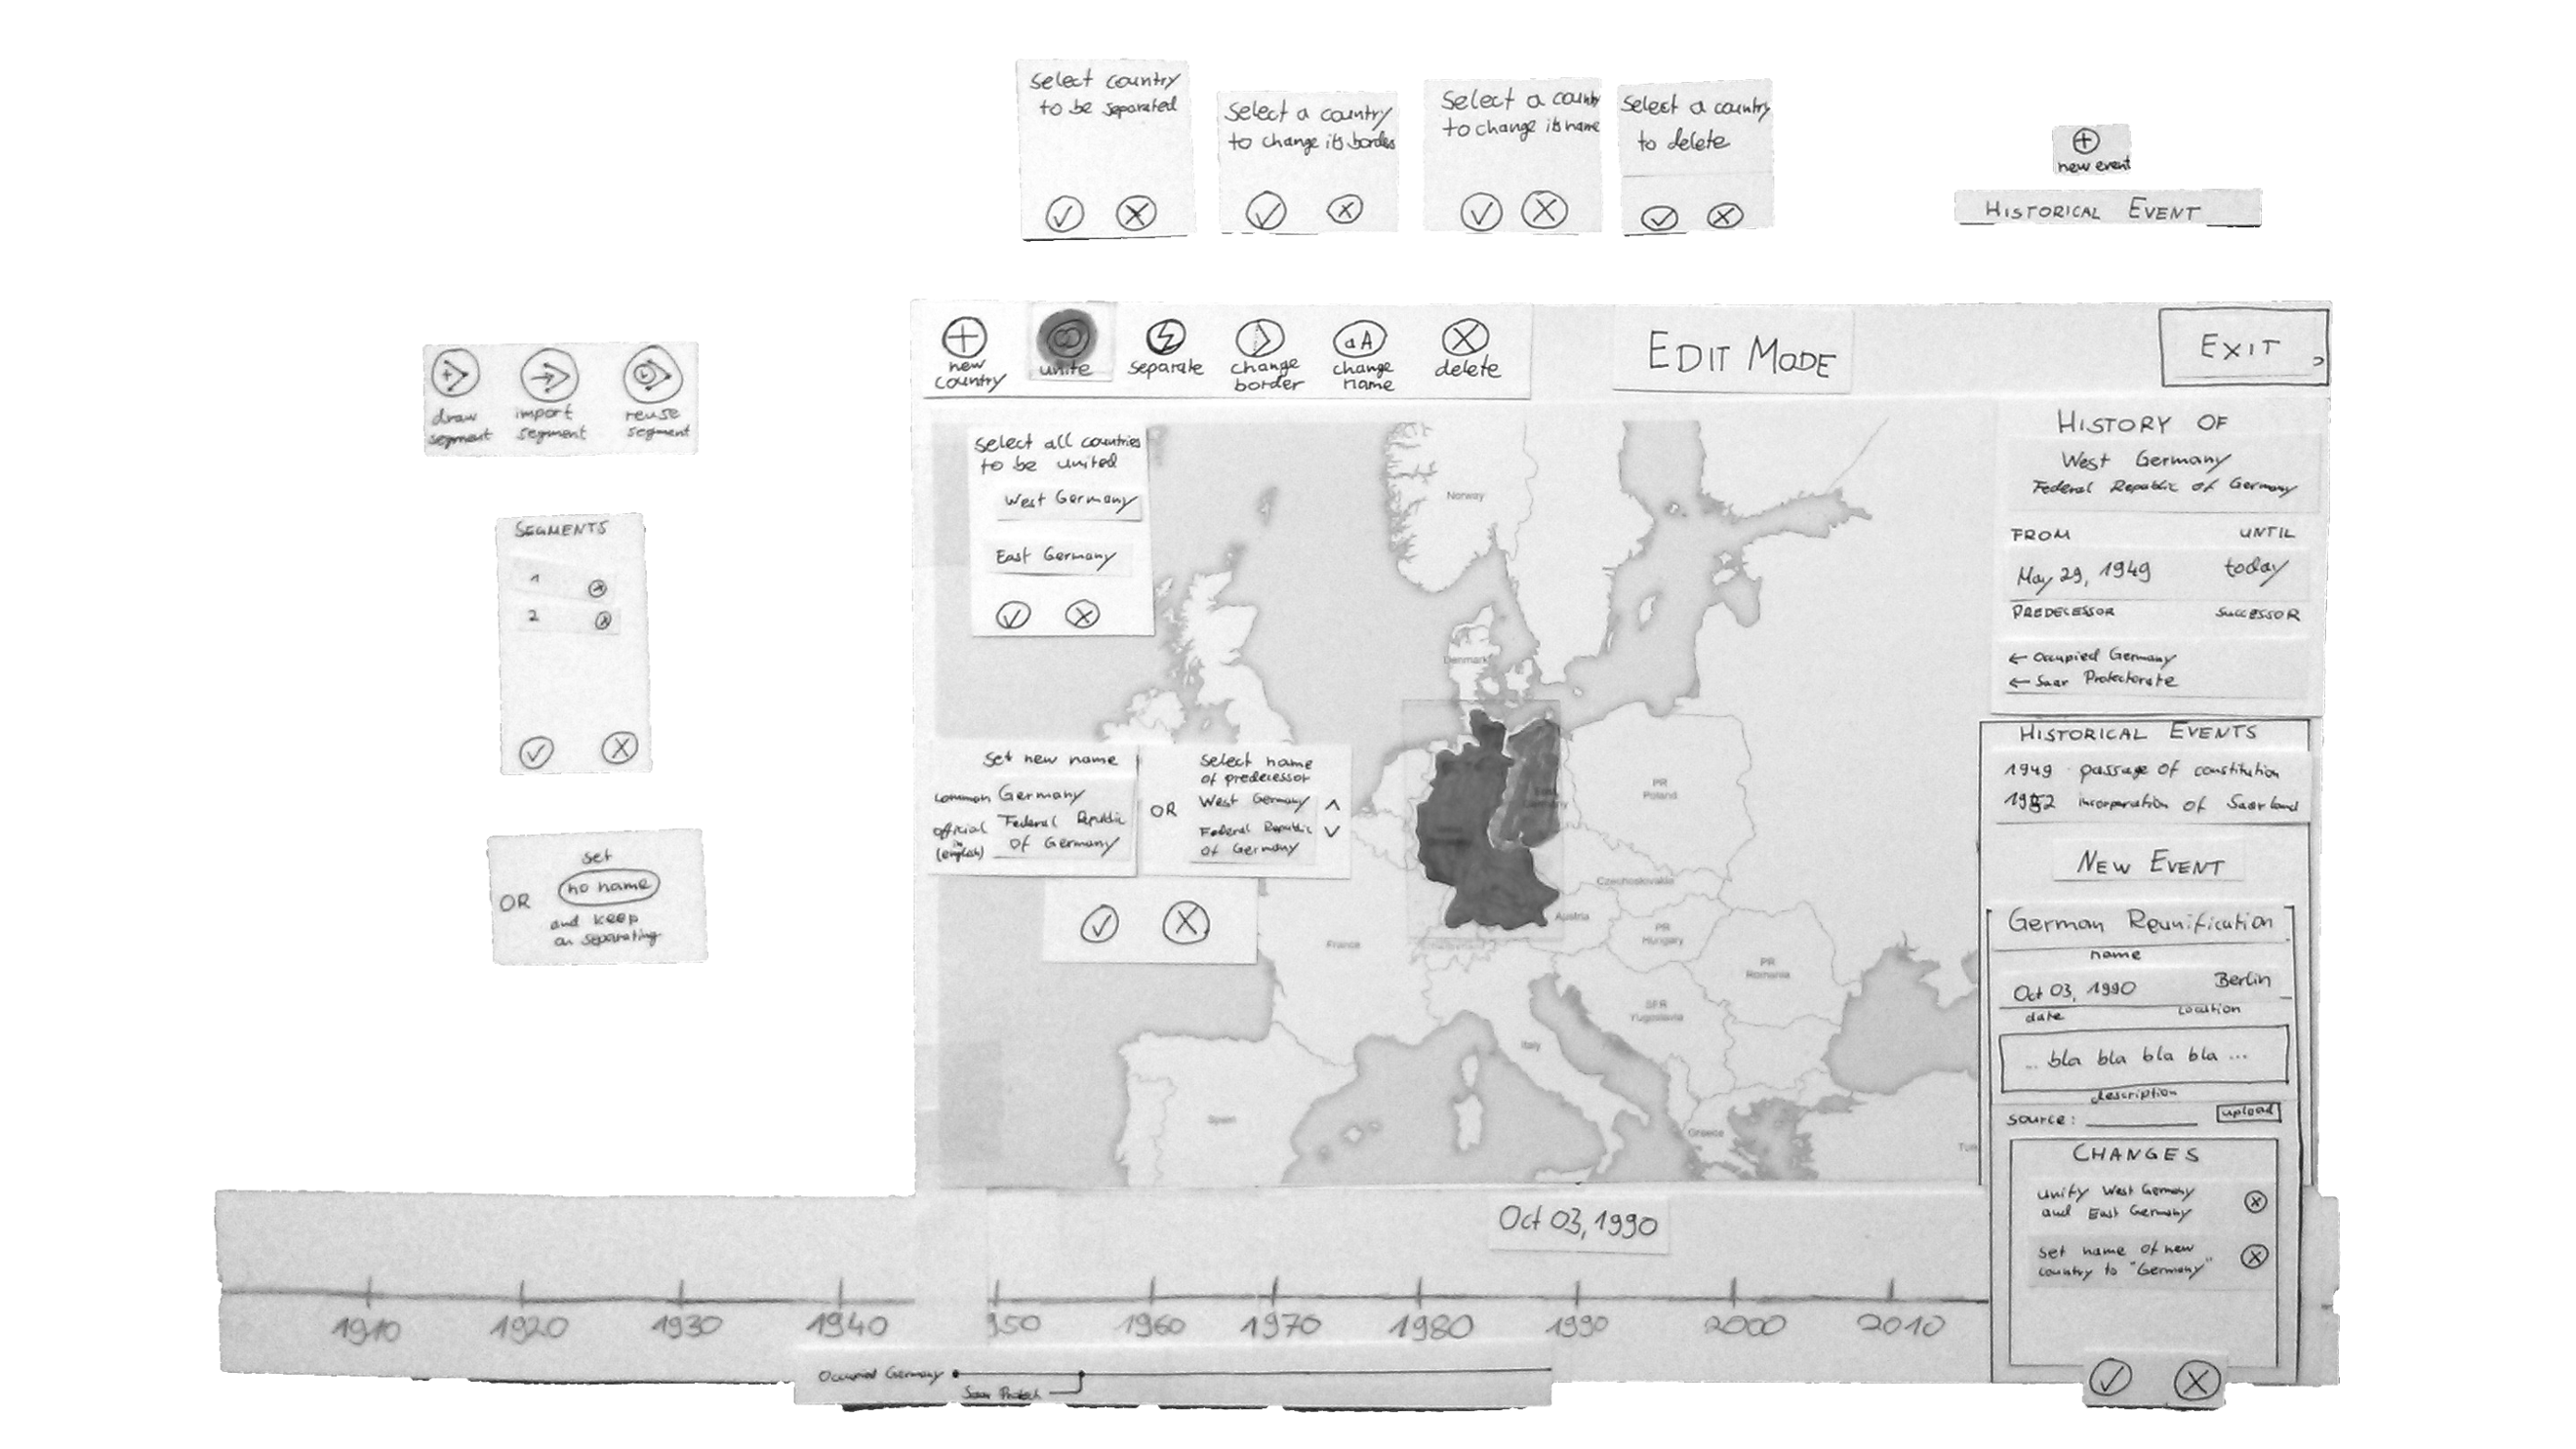
\includegraphics[width=225px]{graphics/development/design_process/paper_prototype_2.png}
\end{subfigure}
\caption{The two iteration of the paper prototype for the Edit Mode}
\label{fig:paper_prototypes}
\end{figure}

The interface consists of a map of Europe, a timeline centered at 1975 and the buttons with a set of dialogs for the for the Edit Mode. Both prototypes were evaluated with three test subjects that had to solve four tasks covering different use cases and operations:
\begin{compactenum}
  \item 1300: Rename incorrectly spelled name of Switzerland on the map (\emph{correction})
  \item 1990: Unite East and West Germany (\emph{forward change})
  \item 1993: Separate the Soviet Union into Russia, Estonia, Latvia, etc. (\emph{forward change})
  \item 1944: Change the border between Finland and the Soviet Union before 1944 (\emph{backward change})
\end{compactenum}

Most parts of the interface concept were understood and all subjects could solve the first three tasks. However, there were also problems:

\begin{compactenum}
  \item There difference between Hivents, the history of a country and an historical change was unclear.
  \item The border drawing dialoge was imagined to be very complex.
  \item The backward change was not understood
  \item Correcting the name Switzerland by changing the event that created it in 1300 caused confusion.
\end{compactenum}

The main finding of this step was that depending on the task, there is both an Hivent-based and an Area-based mental model of the task. This became apparent in the German Reunification Hivent: Some users started the unification operation first, and added West and East Germany afterwards -- and some selected first West Germany, then initiated a unification operation and then added East Germany. From that finding arose that the interface has to support both an Hivent-based and an Area-based approach to introduce historical changes and correct information on the map.

% subsection paper_prototype (end)

% - - - - - - - - - - - - - - - - - - - - - - - - - - - - - - - - - - - - - - -
\subsection{Mockup Prototype} % (fold)
\label{sub:mockup_prototype}

The main part of the design process was spent on the mockup prototypes. Their purpose is to rapidly develop an interface workflow that is understandable by the users. The prototypes were created in \emph{LibreOffice Impress}, an open-source slide-based presentation tool. The interface is simulated on slides: the map is a background image, the timeline, the set of buttons and dialogs for the Edit Mode and HistoGraph are modelled with geometric elements: lines, circles and rectangles. Interactivity is simulated by linking a click on an element to a different slide that shows the effect of the operation. This allows to model sudden changes in the interface.

\begin{figure}[ht]
  \centering
  \begin{subfigure}[b]{.5\textwidth}
    \centering
    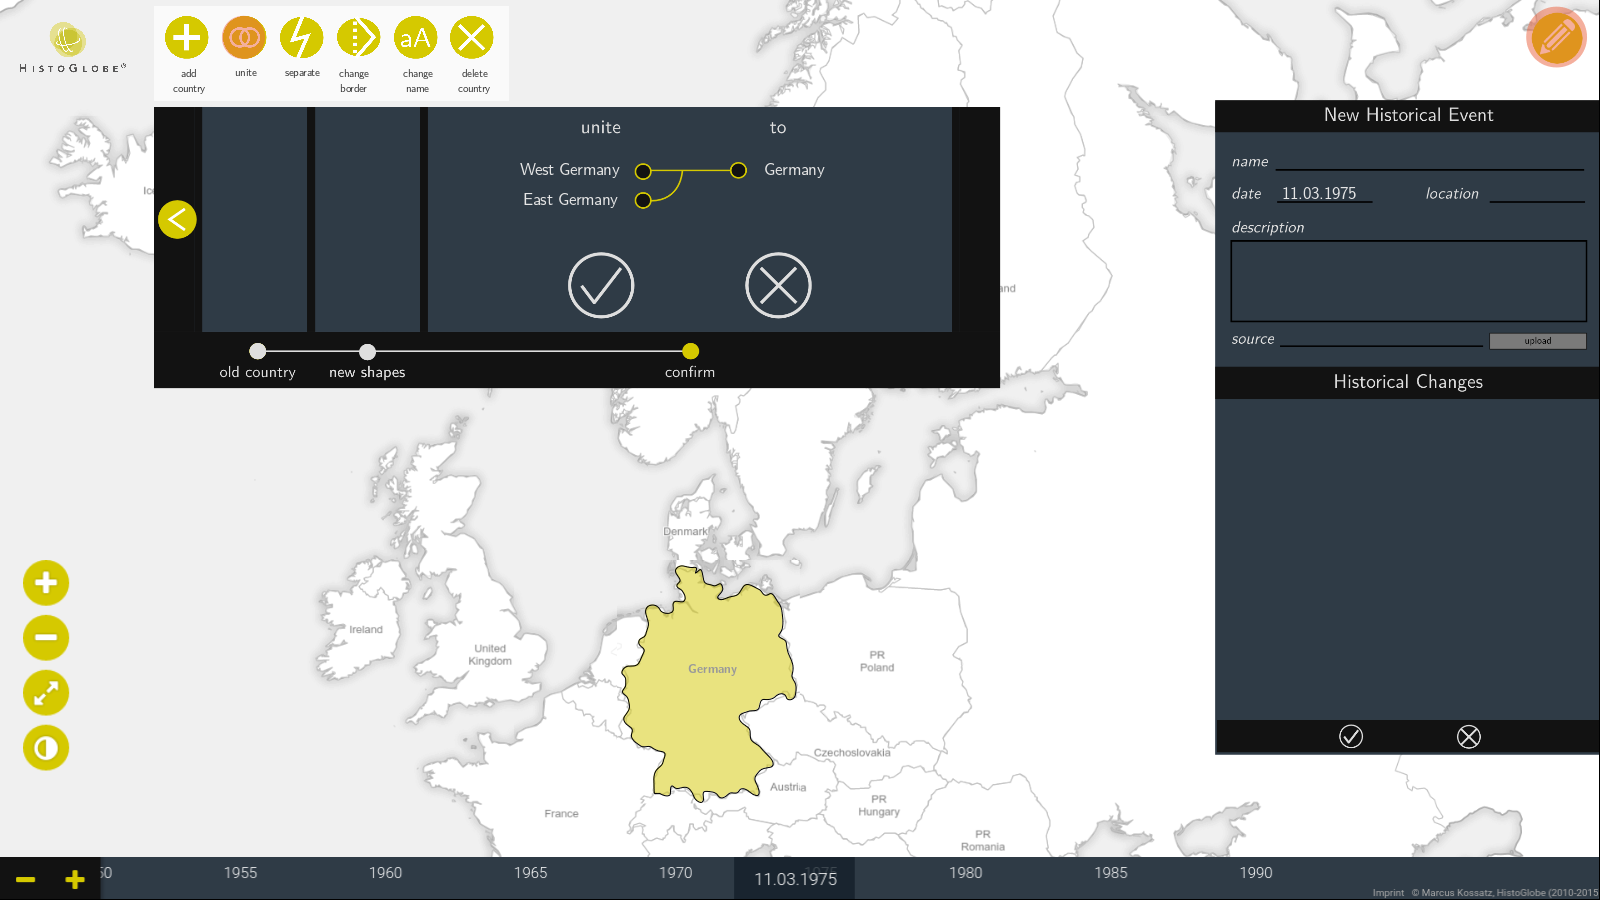
\includegraphics[width=180px]{graphics/development/design_process/mockup_prototype_1.png}
  \end{subfigure}%
  \begin{subfigure}[b]{.5\textwidth}
    \centering
    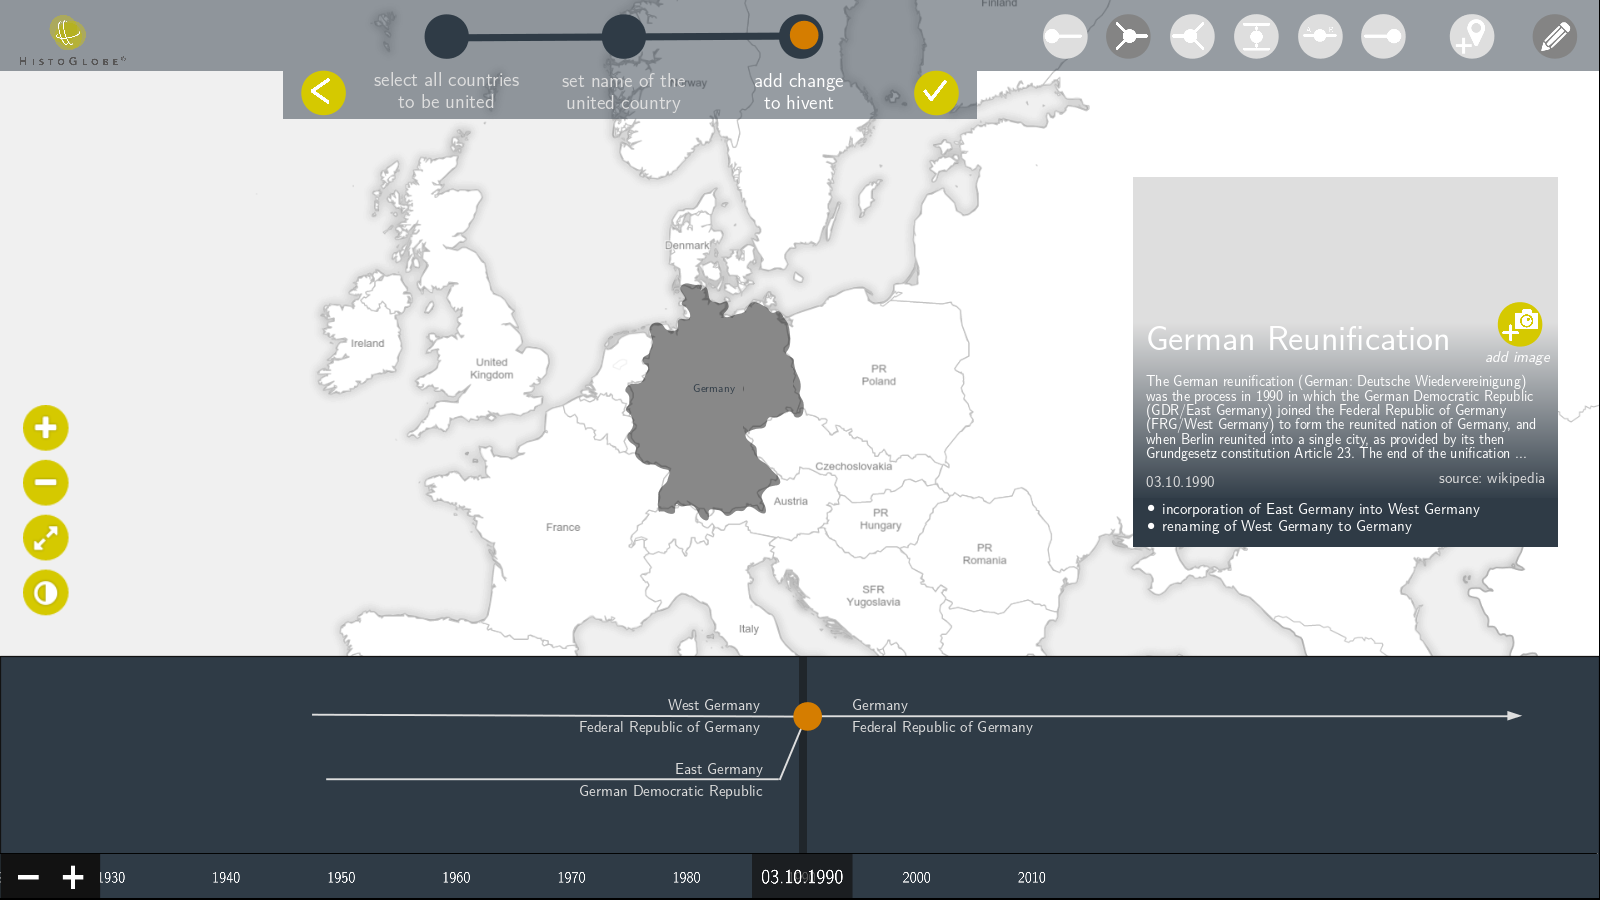
\includegraphics[width=180px]{graphics/development/design_process/mockup_prototype_3.png}
  \end{subfigure} \\[0.8em]

  % \begin{subfigure}[b]{1.0\textwidth}
  %   \centering
  %   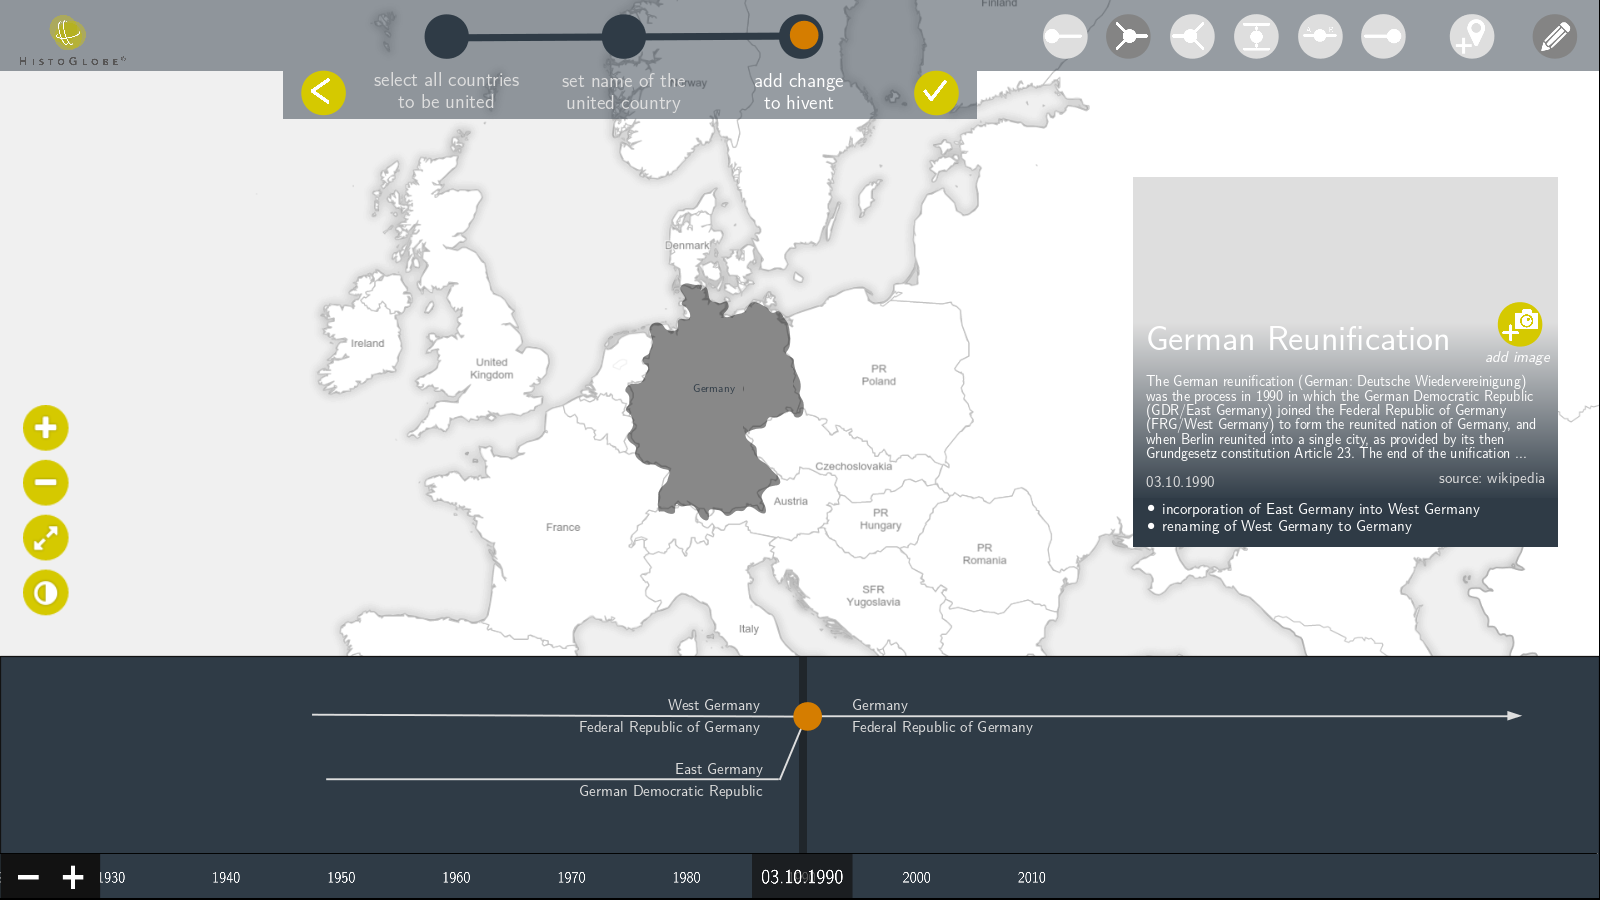
\includegraphics[width=325px]{graphics/development/design_process/mockup_prototype_3.png}
  % \end{subfigure}
  \caption{Two iteration stages of the mockup prototype for the Edit Mode}
  \label{fig:mockup_prototypes}
\end{figure}

Creating the mockup prototype took longer than a paper prototype, but would have still been much faster than actually implementing an interactive Web-based interface. Each prototype iteration was tested with multiple subjects and similar tasks as for the paper prototype. From one test to the next one changes to the interfaces were made. Some interesting quotes from the users were:

\begin{quoteit}
  \begin{tabular}{l r}
    ``this was much easier than I thought'' ~~~~~~~~ &
    ``there is a training session needed'' \\[0.5em]
    ``the interface is very clear &
    ``the logic makes sense, \\
    and graphically pleasing'' &
    it is just very complex'' \\[0.5em]
    ``it's looking good'' &
    ``a nice tutorial and a good \\
    & documentation are necessary'' \\
  \end{tabular}
\end{quoteit}

The main evolution was from a separate dialogue window for the Edit Operation workflow to an intergrated workflow window in the title bar. Also the HistoGraph was introduced to visualize the historical change at while editing it. A lot of smaller design issues, e.g. position of buttons, font sizes or color schemes were identified and fixed. But also conceptual issues arose.

Especially the problem to initiate a backward change (see section \ref{fig:backward_change}) proved to be very difficult. Two design solutions were developed: First, instead of initializing a change in 1990 to separate Germany into East and West, the user can introduce two creation events for the two German states in May and October 1949. The interface needs to provide a visual clue that after creating West Germany, this Area can only be active until 1990, because then another Area, present-day Germany, uses its territory (see figure \ref{sfig:backward_change_1}). The change from West Germany to Germany will be created automatically. The second approach is to introduce a button that flippes an Edit Operation that has just been created (see figure \ref{sfig:backward_change_2}) -- in this case the \texttt{DIS} operation introduced to secede East Germany from Germany will be flipped into a \texttt{UNI} operation to incorporate East Germany into Germany. This approach makes use of the fact that each Edit Operation and has an inverse, as explained in section \ref{par:inverse_operations}.
However, this flipping requires the introduction of additional creation events: West and East Germany were introduced in the change, but only the event that ceases both of them (\texttt{INC} of West Germany into East Germany). They also need a creation event, otherwise they would be active backwards all the way to $t_0$, the initial state of the system.

\begin{figure}[ht]
\centering
\begin{subfigure}[b]{.5\textwidth}
  \centering
  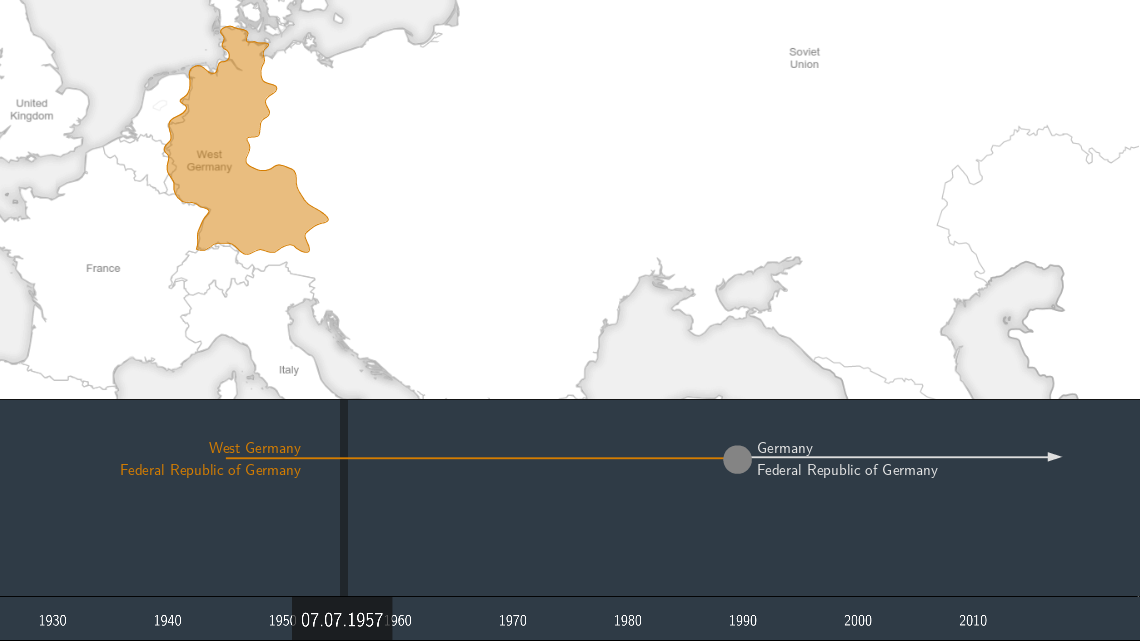
\includegraphics[width=200px]{graphics/development/design_process/backward_change_1.png}
  \caption{Visual clue: predefined and of Area}
  \label{sfig:backward_change_1}
\end{subfigure}%
\begin{subfigure}[b]{.5\textwidth}
  \centering
  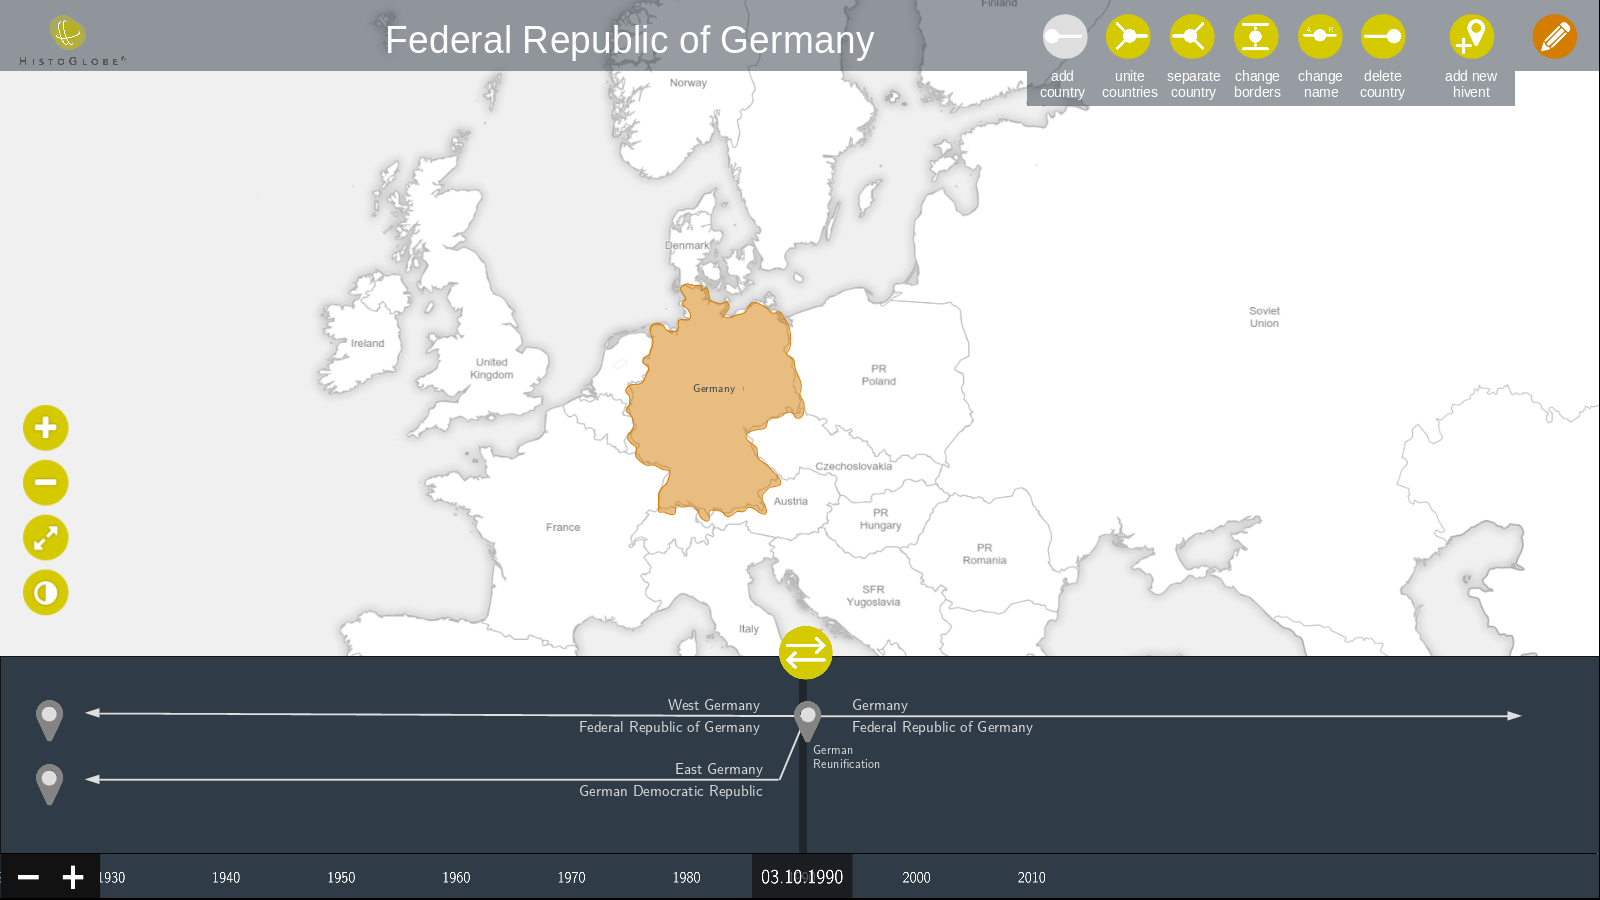
\includegraphics[width=200px]{graphics/development/design_process/backward_change_2.png}
  \caption{Create backward change by flipping Edit Operation}
  \label{sfig:backward_change_2}
\end{subfigure}
\caption{Two approaches for editing changes backwards}
\label{fig:backward_change}
\end{figure}

The prototype was very valuable for the development process. In a total of two weeks, an interface concept and workflow was designed that proved to be understandable by the users.


% subsection mockup_prototype (end)

% - - - - - - - - - - - - - - - - - - - - - - - - - - - - - - - - - - - - - - -
\subsection{Web-based prototype} % (fold)
\label{sub:web_based_prototype}

The main advantage of the design process is that it prevents major redesigns of the final Web-based prototype. After three months of implementation of the final system, the interface looks very similar to the last version of the mockup prototype. The original main elements of the interface are the map, the timeline with the Now Marker indicating the current date of the visualization and the control buttons for zooming the map and the timeline. They are preserved and extended by new interface elements for the Edit Mode. Their interaction and behavior are introduced in this section at the example of the fictional secession of Scotland from the United Kingdom in 2018. The HistoGraph was not implemented, because of the conceptual problems mentioned in section \ref{sub:histograph} that have to be solved first.

\newpage
\begin{minipage}[t]{0.47\textwidth}

  \begin{figure}[H]
    \centering
    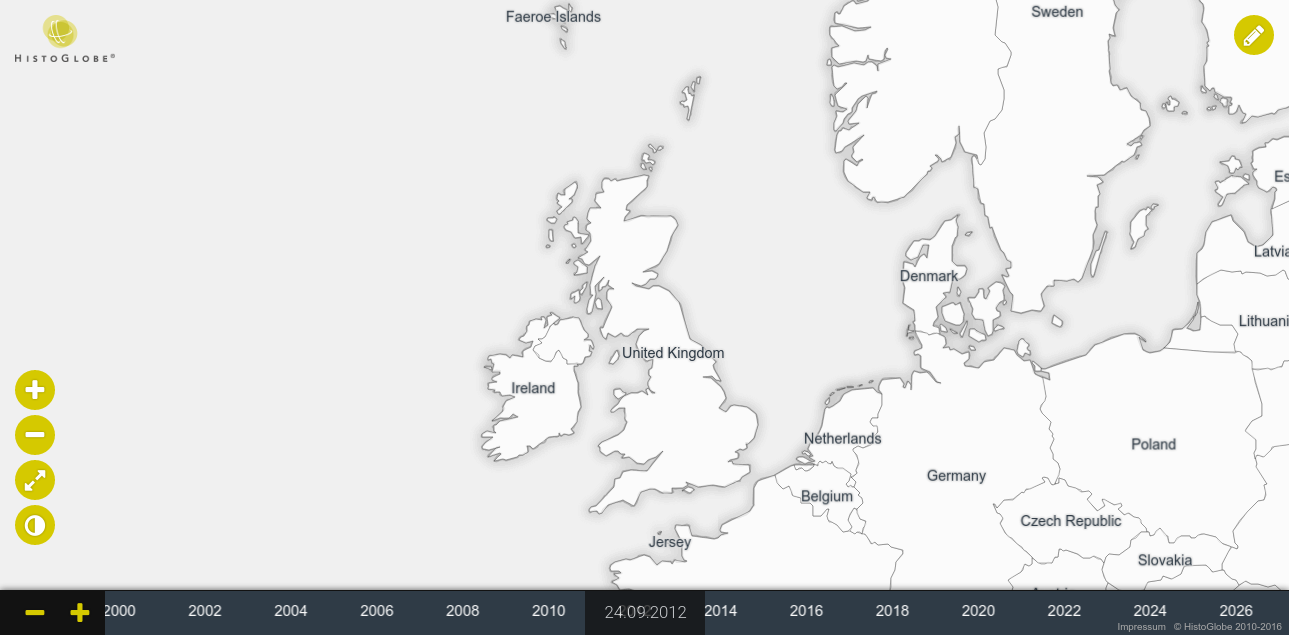
\includegraphics[width=1.0\textwidth]{graphics/development/final_interface/1_init.png}
    \caption{Initial state of the normal mode}
    \label{fig:final_1_init}
  \end{figure}

  The initial state of the user interface. Additional to the original elements, there is an edit button on the upper right corner. Clicking it enters the Edit Mode of the system.

\end{minipage}    % N.B. the % is very important
\hspace{1.5em}    % N.B. this must go in this line, no blank lines !!!
\begin{minipage}[t]{0.47\textwidth}

  \begin{figure}[H]
    \centering
    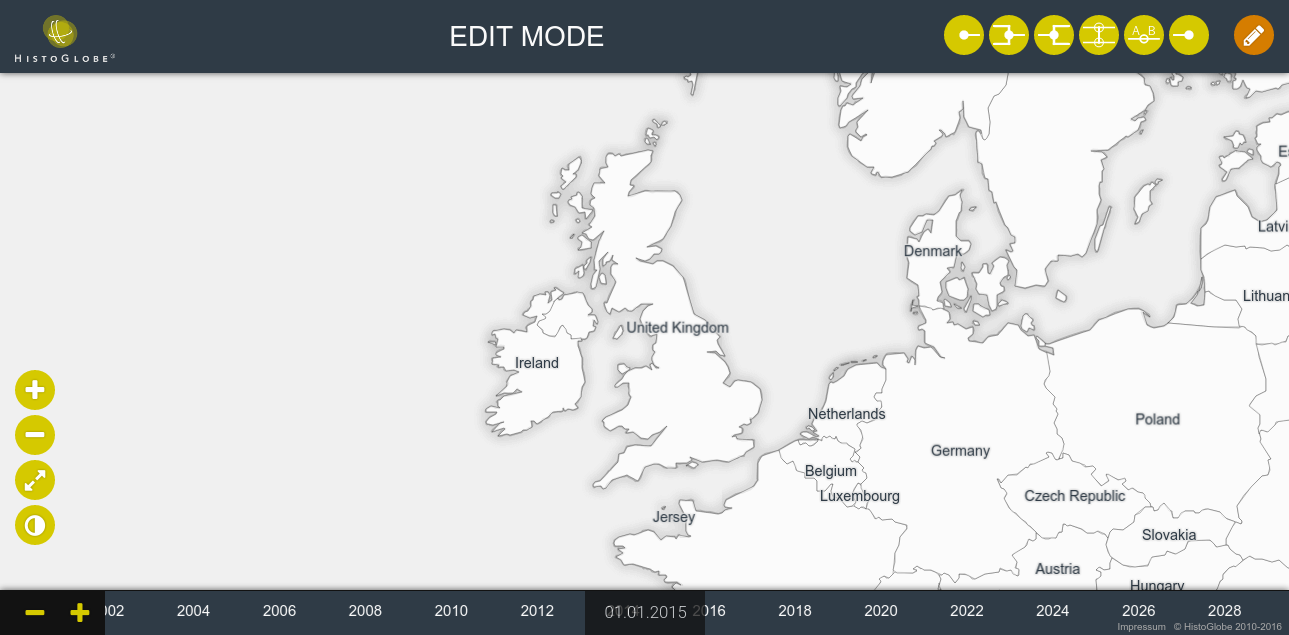
\includegraphics[width=1.0\textwidth]{graphics/development/final_interface/2_edit_mode.png}
    \caption{Initial state of the Edit Mode}
    \label{fig:final_2_edit_mode}
  \end{figure}

  In the Edit Mode, a title bar and six buttons for the Edit Operations are   revealed. Clicking a button starts the operation workflow introduced in section \ref{par:workflow}.

\end{minipage}

\vspace{1em}
\begin{minipage}[t]{0.47\textwidth}

  \begin{figure}[H]
    \centering
    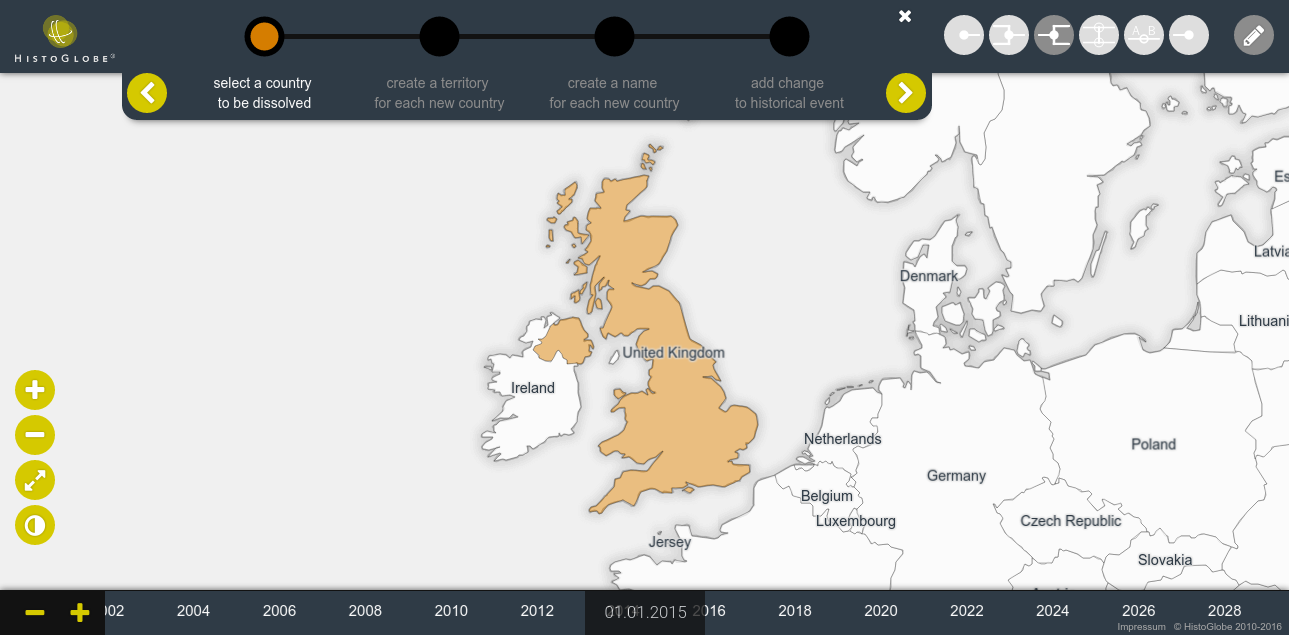
\includegraphics[width=1.0\textwidth]{graphics/development/final_interface/3_select_old_areas.png}
    \caption{Step 1) \texttt{SELECT\_OLD\_AREAS}}
    \label{fig:final_3_select_old_areas}
  \end{figure}

  A \emph{Workflow Window} is guiding the user through the process of completing the historical change. It shows all the steps necessary for this Edit Operation. In the case of \texttt{DIS}, the user has to select the country to be dissolved by clicking it on the map. After the step is completed, clicking the next button in the workflow window procceeds to the next step. At each point in the workflow, clicking the back button reverts the previous action.

\end{minipage}    % N.B. the % is very important
\hspace{1.5em}    % N.B. this must go in this line, no blank lines !!!
\begin{minipage}[t]{0.47\textwidth}

  \begin{figure}[H]
    \centering
    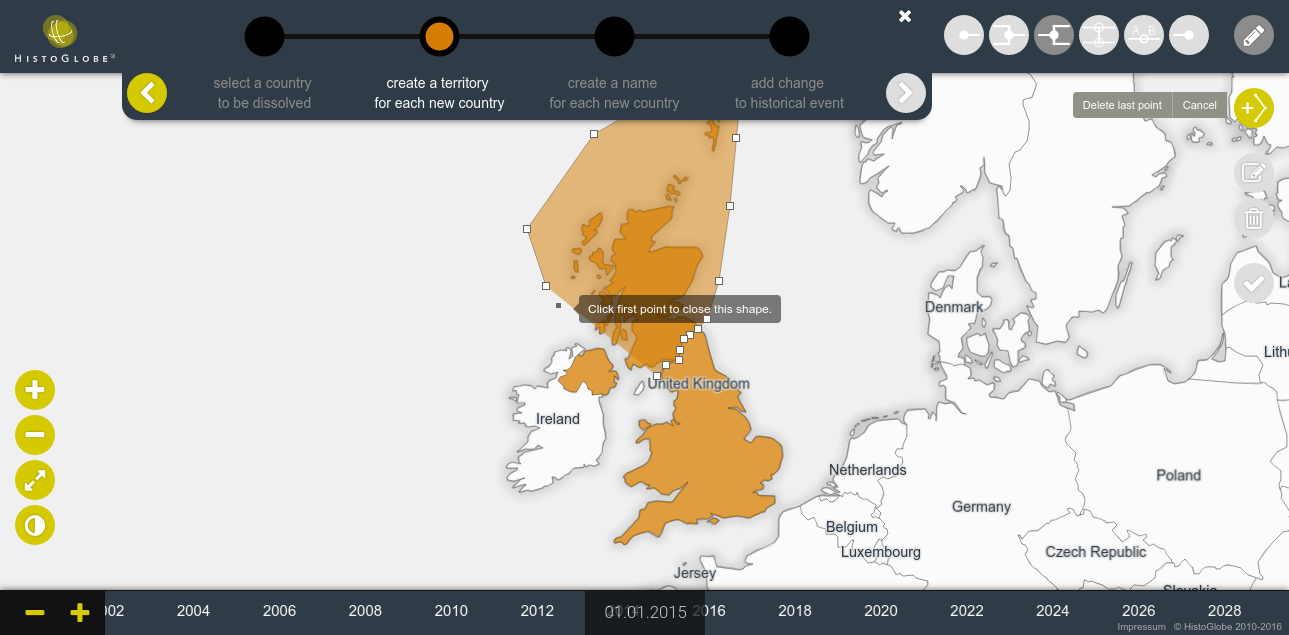
\includegraphics[width=1.0\textwidth]{graphics/development/final_interface/4_set_new_territories.png}
    \caption{step 2) \texttt{SET\_NEW\_TERRITORIES}}
    \label{fig:final_4_set_new_territories}
  \end{figure}

  In the second step, the user has to create the territory for each new Area that shall be created. Therefore, the \emph{New Territory Tool} provides the functionality to create, manipulate and delete polylines by clicking and moving it directly on the map. The polypolygon drawn by the user is intersected with the old territory to create the territory of the new Area. After one new territory is created sucessfully, the second one can be taken from the remaining old territory by selecting it from the map. As soon as the whole old territory is distributed among the new Areas, the workflow proceeds to the next step.

\end{minipage}

\vspace{1em}
\begin{minipage}[t]{0.47\textwidth}

  \begin{figure}[H]
    \centering
    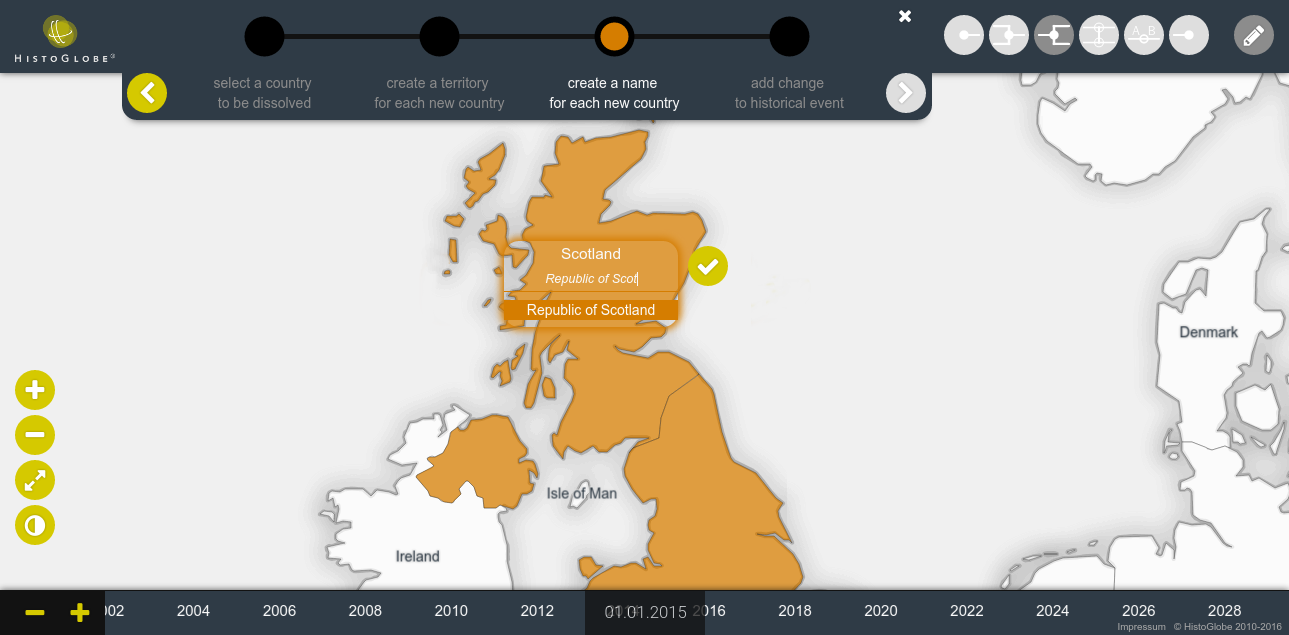
\includegraphics[width=1.0\textwidth]{graphics/development/final_interface/5_set_new_name.png}
    \caption{Step 3) \texttt{SET\_NEW\_NAMES}}
    \label{fig:final_5_set_new_name}
  \end{figure}

  In the next step, for each Area that has been created in the step before, a name has to be defined. The \emph{New Name Tool} is a draggable input form with two lines, the upper one for the short name, the lower one for the formal name, the identity of the Area. Via instant search, the user can select existing country names from the database to be put in the New Name Tool. When clicking the confirm button, the short name is put directly on the map.

\end{minipage}    % N.B. the % is very important
\hspace{1.5em}    % N.B. this must go in this line, no blank lines !!!
\begin{minipage}[t]{0.47\textwidth}

  \begin{figure}[H]
    \centering
    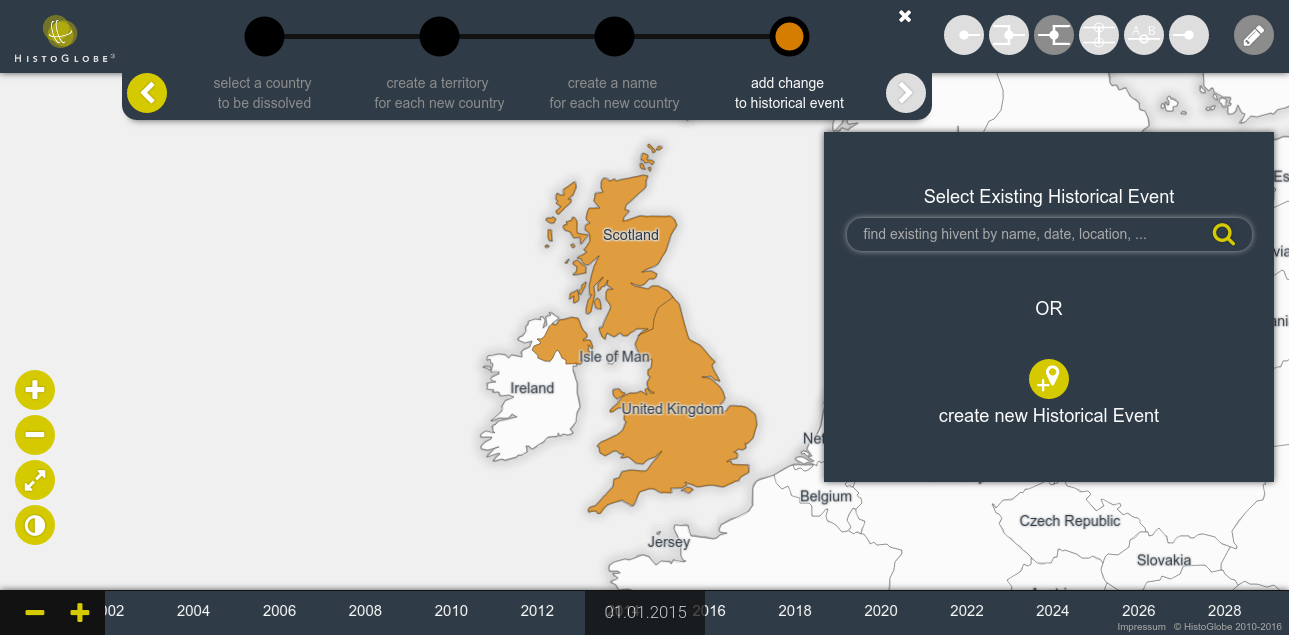
\includegraphics[width=1.0\textwidth]{graphics/development/final_interface/6_add_change_to_hivent_1.png}
    \caption{Step 4) \texttt{ADD\_CHANGE}}
    \label{fig:final_6_add_change_to_hivent_1}
  \end{figure}

  When all names are set, the Edit Operation is complete. In the last step of the workflow, it has to be added to an Hivent. The \emph{New Hivent Box} offers two possibilities: the user can search for an existing Hivent and add the historical change to it, or create a new one.

\end{minipage}

\vspace{1em}
\begin{minipage}[t]{0.47\textwidth}

  \begin{figure}[H]
    \centering
    \includegraphics[width=1.0\textwidth]{graphics/development/final_interface/7_add_change_to_hivent_2.png}
    \caption{Step 4) \texttt{ADD\_CHANGE}}
    \label{fig:final_7_add_change_to_hivent_2}
  \end{figure}

  The new Hivent created for that change is the ``Scottish Independence'' on 01.01.2018 with a description of the Hivent and possibly a location and a link to a wikipedia article. In the last line, the historical change ``Secession of Scotland from the United Kingdom'' is noted. Clicking the confirm button finalizes the workflow.

\end{minipage}    % N.B. the % is very important
\hspace{1.5em}    % N.B. this must go in this line, no blank lines !!!
\begin{minipage}[t]{0.47\textwidth}

  \begin{figure}[H]
    \centering
    \includegraphics[width=1.0\textwidth]{graphics/development/final_interface/8_final_state.png}
    \caption{The final state with Scotland}
    \label{fig:final_8_final_state}
  \end{figure}

  Clicking the edit button again leaves the Edit mode back to the normal view. Scotland and the United Kingdom are both visible on the map after 2018. When moving the timeline before 2018, Scotland is still part of the UK.

\end{minipage}

% subsection web_based_prototype (end)

% section user_interface_design_process (end)
%!TEX root = ../masters_thesis.tex

\section{Application} % (fold)
\label{sec:application}

HistoGlobe is a Web-based Historical Geographic Information System. The Data model and the conceptual model of the user interface were introduced in the first sections of this chapter. This section introduces the underlying database model, a specific implementation of the data model, and the computational model that translates between the conceptual model and the database model. The first part provides an overview about the architecture of the system in section \ref{sub:system_architecture}.
% ... bla bla bla, the rest comes last
% problems
% - support uncertainty

% ------------------------------------------------------------------------------
\subsection{System Architecture} % (fold)
\label{sub:system_architecture}

HistoGlobe uses a classical client-server architecture of a Web-based information system. The user opens the application and interacts with it through the user interface in a Web browser, the \emph{client} side of the system. The Web \emph{server} is a remote computer that hosts the database and the middleware. The user interacts with the interface and the client-side application sends a request to the Web server for new data. The middleware checks the request and queries the necessary data from the database. It transforms the data and sends it back to the client. The interface shows the new information.

\begin{figure}[H]
  \vspace{1em}
  \centering
  \includegraphics[width=0.7\textwidth]{graphics/development/application/system_architecture}
  \caption{The system architecture of HistoGlobe}
  \label{fig:system_architecture}
\end{figure}

This clear separation between the data, the application and the user interaction in this chapter and in the system follows directly from the \emph{model-view-controller} pattern: One part can be changed independently from the others parts: if the 2D map is replaced by a 3D globe, only the view changes, but the middleware and the database can stay untouched. Likewise, the implementation of a new database technology has no consequences to the view.

% subsection system_architecture (end)

% ------------------------------------------------------------------------------
\subsection{Server-Side Application} % (fold)
\label{sub:server_side_application}

The underlying Hivent Model is implemented on the server-side part of the application. HistoGlobe uses \emph{Django}, a free and open-source web framework
\footnote{
  \emph{Django},
  The Web framework for perfectionists with deadlines,
  URL: \url{https://www.djangoproject.com/},
  last access: 27.05.2016
},
combined with \emph{PostgreSQL}
\footnote{
  \emph{PostgreSQL:},
  The world's most advanced open source database,
  URL: \url{http://www.postgresql.org/},
  last access: 31.10.2015
}
, one of the most popular Object-Relational Database Management Systems introduced in section \ref{sub:object_relational_database_management_systems}, on the server-side of the system. This allows HistoGlobe to take advantage of object-oriented concepts in a stable and fast relational database. Since the database is using a lot of geospatial data, \emph{PostGIS} is used as a spatial database extension for PostgreSQL
\footnote{
  \emph{PostGIS},
  Spatial and Geographic Objects for PostgreSQL,
  URL: \url{http://postgis.net/},
  last access: 27.05.2016
}.

With these tools at hand, the Hivent Model form section \ref{sec:hivent_model}  was implemented in a database model shown in figure \ref{fig:database_model_er}. It is the final result of a highly iterative process that underwent many improvements and adpations to new requirements introduced in the Human Centered Design process. The model is structured in two parts covereing four different domains of the spatio-temporal model: The lower part describes the semantic, spatial and thematic domain of Areas and the upper part represents the temporal domain of Hivents that introduces changes to the Areas.

\begin{figure}[ht]
  \centering
  \includegraphics[width=0.8\textwidth]{graphics/development/application/database_model}
  \caption{The Hivent Database Model}
  \small{Each entity additionally has an \texttt{id} attribute, which is omitted for simplification purposes.}
  \label{fig:database_model_er}
\end{figure}

% - - - - - - - - - - - - - - - - - - - - - - - - - - - - - - - - - - - - - - -
\paragraph{Semantic, Spatial and Thematic Domain} % (fold)
\label{par:semantic_spatial_and_thematic_domain}

In the Hivent Model, the entity visible on the map is an Area with a name and a territory, as introduced in section \ref{sec:hivent_model}. In the database model, they are represented by three entities:

\begin{enumerate}
  \item \texttt{Area}: semantic domain defining one identical Area with potentially changing name and territory. The \texttt{universe} attribute is true for $\Omega$, for the other Areas it is false.
  \item \texttt{AreaTerritory}: spatial domain. A polypolygon describes the \texttt{geometry} of the territory and a \texttt{representative\_point} the position of the name label on the map.
  \item \texttt{AreaName}: thematic domain. It is defined by a \texttt{short\_name} and a \texttt{formal\_name}.
\end{enumerate}

% paragraph semantic_spatial_and_thematic_domain (end)

% - - - - - - - - - - - - - - - - - - - - - - - - - - - - - - - - - - - - - - -
\paragraph{Temporal Domain} % (fold)
\label{par:temporal_domain}

The main idea of the model is that the Areas can change over time. These changes are introduced by \texttt{Hivents}, the main entitity of the eponymic model with five attributes: The \texttt{name} and a textual \texttt{description} of the Hivent, the point in time the Hvent happend (\texttt{date}), the Hivent \texttt{location} as a simple string and a \texttt{link} (URL) to the related article, serving as a historical source. Each Hivent can introduce a set of \texttt{EditOperation}s introduced and understood by the user. They consist themselves of a set of low-level \texttt{HiventOperation}s). They replace a set of \texttt{OldArea}s with a set of \texttt{NewArea}s and might update the name or the territory of one specific \texttt{UpdateArea}.

% paragraph temporal_domain (end)

% - - - - - - - - - - - - - - - - - - - - - - - - - - - - - - - - - - - - - - -
\paragraph{Example} % (fold)
\label{par:example}

Figure \ref{fig:database_example_reunification} shows the Hivent Database Model at the example of the German Reunification on 3. October 1990. Before 1990, there were the Areas \texttt{GDR} (``German Democratic Republic'', East Germany) and \texttt{FRG} (``Federal Republic of Germany'', West Germany). A user introduced a Merge operation (\texttt{MRG}) in the Edit Mode between \texttt{FRG} and \texttt{GDR}. The new Area received the short name ``Germany'' and the same formal name ``Federal Republic of Germany'' as previous West Germany. Internally, the Edit Mode translates this to an \texttt{INC} of \texttt{GBDR} into \texttt{FRG} and a subsequent \texttt{NCH} of the \texttt{FRG}. One Area ceases, one Area is updated twice and no new Area is created.

\begin{figure}[ht]
  \vspace{1em}
  \includegraphics[width=0.9\textwidth]{graphics/development/application/example_reunification}
  \caption{Visualization of the German Reunification in the Hivent Database Model}
  \label{fig:database_example_reunification}
\end{figure}


% paragraph example (end)

% - - - - - - - - - - - - - - - - - - - - - - - - - - - - - - - - - - - - - - -
\paragraph{Initial Dataset} % (fold)
\label{par:initial_dataset}

Section \ref{sub:data_sources} explained the lack of data about historical countries. It is out of the scope of this thesis to create a large testing dataset with the historical countries in the world. The inital dataset consists of the following countries, their names and borders: the 193 UN members and 2 observer states (created by \texttt{CRE} operation) and seven countries with limited international recognition: Kosovo, Transnistria, South Ossetia, Abkhazia, Nagorno-Karabakh, Somaliland and Sahrawi Arab Democratic Republic, see section \ref{par:un_non_members_with_limited_recognition}) (created by \texttt{DIS} operations from their homeland on the day of their declaration of independence).

% paragraph initial_dataset (end)

% - - - - - - - - - - - - - - - - - - - - - - - - - - - - - - - - - - - - - - -
\paragraph{Middleware} % (fold)
\label{par:middleware}

The Django web framework provides \emph{view} classes as the middleware that receives requests from the client, processes them, queries the necessary data from the database and returns an \texttt{HttpResponse} back to the client. In the naive implementation of the system, the middleware provides only two views for the two use cases:

\begin{enumerate}
  \item \textbf{\texttt{get\_all}} is initially called by the client side on loading the web service. The server responds to this \texttt{HttpRequest} with all data from the database in one \emph{JSON} object. While this behaviour is not scalable, for the initial dataset it was sufficient: The data was loaded in 3.5 seconds.
  \item \textbf{\texttt{save\_edit\_operation}} is called by the client after an Edit Operation has been completely created in the Edit Mode. In the last step, the client assembles the relevant data: the associated \texttt{Hivent} and \texttt{HiventOperation}s), data about each \texttt{OldArea}, \texttt{UpdateArea} and \texttt{NewArea}. The view checks the data for integrity and stores them in the database. The method returns to the client a confirmation and a set of final \texttt{id}s for the entities stored in the database.
\end{enumerate}

% paragraph middleware (end)

% subsection server_side_application (end)

% ------------------------------------------------------------------------------
\subsection{Client-Side Application} % (fold)
\label{sub:client_side_application}

The main application of HistoGlobe runs on the client. As introduced in section \ref{sec:histoglobe}, the software is built upon a module system. The modules used in this this implementation of HistoGlobe are emphazised in \textbf{bold} in the class diagram in figure \ref{fig:class_diagram}. The classes are structured by their functionality regarding the Model-View-Controller pattern.

\begin{sidewaysfigure}[p]
  \centering
  \includegraphics[width=0.95\textwidth]{graphics/development/application/class_diagram}
  \vspace{1em}
  \caption{Class Diagram of HistoGlobe}
  \label{fig:class_diagram}
\end{sidewaysfigure}

\newpage % forces the figure to be on the next page, because [H] does not work
% - - - - - - - - - - - - - - - - - - - - - - - - - - - - - - - - - - - - - - -
\paragraph{Initialization} % (fold)
\label{par:initialization}

The main HistoGlobe instance in the bottom initializes all modules, mainly the interface elements, the controllers and the \texttt{DatabaseInterface}. This class communicates with the middleware (section \ref{par:middleware}), loads data from and stores data in the database. Initially, each \texttt{Hivent} and the related \texttt{EditOperation}s and \texttt{HiventOperation}s are created. Each \texttt{HiventOperation} is assembled by its associated set of \texttt{OldArea}s, \texttt{NewArea}s and the \texttt{UpdateArea} from the datase model in  figure \ref{fig:database_model_er}. Afterwards, each \texttt{Area}, \texttt{AreaName} and \texttt{AreaTerritory} is loaded. A double-link is established to their associated \texttt{HiventOperation}s via the \texttt{startOperation}, \texttt{updateOperation} and \texttt{endOperation}. Therefore, each \texttt{HiventOperation} knows which \texttt{Area}s, names and territories it creates, updates and ceases -- and vice verse each \texttt{Area}, \texttt{AreaName} and \texttt{AreaTerritory} knows which \texttt{HiventOperation} manipulates its evolution.

% paragraph initialization (end)

% - - - - - - - - - - - - - - - - - - - - - - - - - - - - - - - - - - - - - - -
\paragraph{Executing temporal changes} % (fold)
\label{par:executing_temporal_changes}

HistoGlobe visualizes time on the interactive \texttt{Timeline} and the static \texttt{NowMarker} showing the current date of the application: the \texttt{NowDate}. Both view classes can manipulate the current date by moving the \texttt{Timeline} or entering a date into the \texttt{NowMarker}. The \texttt{TimeController} stores the \texttt{NowDate} and tells all other modules if the current visualization has changed.

\begin{figure}[ht]
  \vspace{1em}
  \centering
  \includegraphics[width=0.8\textwidth]{graphics/development/application/hivent_controller}
  \caption{Detecting the next Hivent that happens in the \texttt{HiventController}}
  \label{fig:hivent_controller}
\end{figure}

The core of the Hivent-based implementation is the \texttt{HiventController}. Figure \ref{fig:hivent_controller} illustrates how it works: The controller stores a reference to each \texttt{Hivent} chronologically in a doubly-linked list, i.e. each \texttt{Hivent} knows the historically next and previous \texttt{Hivent}. Additionally, the controller stores a pointer to the last \texttt{Hivent} in the list that has happened and a copy of the current date. It listens to the \texttt{TimeController} -- if the \texttt{NowDate} changes, the \texttt{HiventController} checks for the next \texttt{Hivent} if it has happened: The controller compares this new date with its current date checks if the \texttt{Hivent.date} is in between these two dates. If this is the case, the \texttt{Hivent} happens and all the \texttt{EditOperations} associated to this \texttt{Hivent} are executed on the map. The \texttt{HiventController} updates the pointer to the \texttt{Hivent} and checks for the next one until the next \texttt{Hivent} is outside this time span. If the \texttt{nowDate} from the \texttt{TimeController} is before the current date of the \texttt{HiventController}, it checks for \texttt{Hivents} backwards through the list and executes all the \texttt{EditOperations} backwards. This simple data structure allows to effectively and efficiently manage temporal changes of \texttt{Area}s on the map. On initialization of the system, after the \texttt{DatabaseInterface} loaded all the data, the \texttt{HiventController} starts this process: All \texttt{Hivent}s in the list from the beginning until the \texttt{NowDate} of the \texttt{TimeController} are happening one after the other.

An \texttt{EditOperation} diverts the execution to all its related \texttt{HiventOperations}. They are the integral objects that change the status on the map. The main part of its source code, the \texttt{execution} function is shown in listing \ref{lst:hivent_operation}. As mentioned above, there are two change directions: forward and backward. If an \texttt{HiventOperation} is to be executed forwards, the following three steps happen:

\begin{enumerate}
  \item For each \texttt{newArea}, the \texttt{AreaName} and the \texttt{AreaTerritory} that the \texttt{Area} has in the moment it gets historically created are associated to the \texttt{Area}. Afterwards, the \texttt{Area} is shown on the map: The \texttt{AreaHandle} associated to the \texttt{Area} has a function that tells the \texttt{AreaNameLayerOnMap} and \texttt{AreaTerritoryLayerOnMap} to be shown.
  \item For each \texttt{oldArea}, the opposite happens: the name and territory are detached from the \texttt{Area} and the \texttt{AreaHandle} hides the \texttt{Area} from the map.
  \item In the \texttt{updateArea} the \texttt{AreaName} or \texttt{AreaTerritory} is replaced by the \texttt{newName} respectively \texttt{newTerritory}. The \texttt{update} method of the \texttt{AreaHandle} updates the respective layers on the map.
\end{enumerate}

In case the operation happens backwards, \texttt{oldAreas} and \texttt{newAreas} are swapped and the \texttt{updateArea} uses the \texttt{oldName} respectively \texttt{oldTerritory} instead.

\begin{center}
\begin{minipage}[t]{0.8\textwidth}
\begin{lstlisting}[language=coffeescript,
  caption=Execution of an \texttt{HiventOperation},
  label=lst:hivent_operation]
class HiventOperation

  constructor: (data) ->
    #...

    @oldAreas   = []  # {area, name, territory}
    @newAreas   = []  # {area, name, territory}
    @updateArea = {}  # {area, oldName, newName, oldTerritory, newTerritory}

    #...

  execute: (direction) ->

    if direction is 1

      for newArea in @newAreas
        newArea.area.name =       newArea.name
        newArea.area.territory =  newArea.territory
        newArea.area.handle.show()

      for oldArea in @oldAreas
        oldArea.area.name =       null
        oldArea.area.territory =  null
        oldArea.handle.hide()

      if @updateArea
        if @updateArea.newName
          @updateArea.area.name =      @updateArea.newName
        if @updateArea.newTerritory
          @updateArea.area.territory = @updateArea.newTerritory
        @updateArea.area.handle.update()

    else # direction is -1 => backward change
      # same as above, just each 'new' is replaced by 'old' and vice versa
\end{lstlisting}
\end{minipage}
\end{center}

% paragraph executing_temporal_changes (end)

% - - - - - - - - - - - - - - - - - - - - - - - - - - - - - - - - - - - - - - -
\paragraph{EditMode} % (fold)
\label{par:editmode}

The Edit Mode is the main contribution of this thesis to the HistoGlobe project. Its interface was introduced in section \ref{sub:web_based_prototype}, this section shortly explains its implementation: When the user clicks a button of an Edit Operation in the upper right corner of the Edit Mode interface, internally a \texttt{EditOperationCreator} sets up the \texttt{WorkflowWindow} in the interface and the first \texttt{EditOperationStep} for this operation. Each of the four steps have different tasks. They area introduced in section \ref{sub:edit_workflow}. The \texttt{EditOperationCreator} stores the data for each step (selected Areas, newly defined territories and names) in an object. Each step can access this object and manipulate its content. It was especially difficult to design each action to be fully reversible. For that purpose, an associated inverse of the action was stored in an \texttt{UndoManager} that works like a stack. If the user clicks the back button in the Workflow Window, the last action of the stack gets executed. When the last stage of the workflow (\texttt{AddToHivent}) is completed, the \texttt{EditOperationCreator} assembles the \texttt{HiventOperations} from the data gathered in the task. It sends it along with the associated \texttt{Hivent} to the server and finishes the operation.

% paragraph editmode (end)

% - - - - - - - - - - - - - - - - - - - - - - - - - - - - - - - - - - - - - - -
\paragraph{Within-Tree} % (fold)
\label{par:within_tree}

One particular problem of the territory of an Area is that the associated polypolygon can have holes to account for enclaves and exclaves. They can even be nested (second-order enclaves, third-order enclaves, etc.), as in the example of Baarle-Nassau and Baarle-Hertog at the border between the Netherlands and Belgium
\footnote{
  \emph{The Curious Case of Baarle-Nassau and Baarle-Hertog},
  kaushik, 06.11.2012,
  \url{http://www.amusingplanet.com/2012/11/the-curious-case-of-baarle-nassau-and.html},
  last access: 31.05.2016
}.
The \texttt{NewTerritoryTool} has to ensure that the drawn polygons are not self-intersecting and that no two polygons for one territory partially overlap each other. If they fully overlap, then they are holes in the polygon. A polygon consist of one \emph{outer ring}, a closed polyline forming the boundary of the polygon, and a set of \emph{inner rings}, closed polylines defining the holes in the polygon. Second-order enclaves are new polygons that happen to be positioned inside the inner rings of the other polygon. They can themselves have inner rings, which represent third-order enclaves, etc.

In order to supported nested holes, the \emph{WithinTree} is introduced. The idea of the tree is to set up an hierarchical structure of polygons that contain each other. An example Within-Tree for a random set of polygons can be seen in figure \ref{fig:within_tree}.

\begin{figure}[ht]
  \vspace{1em}
  \centering
  \includegraphics[width=0.6\textwidth]{graphics/development/application/within_tree}
  \caption{The Within-Tree (left) for the set of polygons (right)}
  \label{fig:within_tree}
\end{figure}

The algorithm for inserting a polygon as a node into the tree is shown in listing \ref{lst:within_tree_insertion}. After the tree has been set up, the correct structure of polygons can be obtained by traversing the tree in the following custom order:

\begin{compactenum}
  \item Remove the first child $F$ of the root node and all its children $C$ from the tree.
  \item Insert each child of each $C$ as a direct child of the root node.
  \item Create a new polygon with $F$ as the outer ring and each $C$ as an inner ring.
  \item Repeat until the tree is empty.
\end{compactenum}



\begin{center}
\begin{minipage}[t]{0.8\textwidth}
\begin{lstlisting}[language=coffeescript,
  caption=Insertion of a polygon node into the Within-Tree,
  label=lst:within_tree_insertion]
insert: (newNode, parentNode) ->

  ## PREPARATION
  # case 1) newNode also in 1 child of parentNode  -> withinChild
  # case 2) 1+ children of parentNode in newNode   -> containChildren
  # case 3) no hierarchical relation between newNode and any other node

  withinChild =     null
  containChildren = []

  for childNode in parentNode.children

    if newNode.isWithin childNode                   # check if case 1)
      withinChild = childNode
      break # no other hierarchical relation to any other child possible

    else if childNode.isWithin newNode              # check if case 2)
      containChildren.push childNode

  ## EXECUTION

  if withinChild                                    # case 1)
    @insert newNode, childNode

  else                                              # cases 2 and 3)
    # newNode is not in any child of parentNode => place it underneath
    @_nodes.push newNode
    newNode.setParent parentNode
    parentNode.addChild newNode

    for containChild in containChildren             # case 2)
      # => detach from parent node and place them as children of newNode
      containChild.setParent newNode
      newNode.addChild containChild
      parentNode.removeChild containChild
\end{lstlisting}
\end{minipage}
\end{center}

% paragraph within_tree (end)

% - - - - - - - - - - - - - - - - - - - - - - - - - - - - - - - - - - - - - - -
\paragraph{LabelManager} % (fold)
\label{par:labelmanager}

A major visualization problem that was sufficiently solved is the thesis is the label collision problem: Each active Area has both a territory and a name that should be shown on the map. Since no territories can overlap (precondition \ref{axm:unique_coverage}), they can all be shown. This is not true for the names of the Areas: The \texttt{short\_name} of the \texttt{AreaName} is placed as a label in the \texttt{representative\_point} of the \texttt{AreaTerritory}. Labels can overlap, because they can extend beyond their territory. To avoid this, some labels have to be hidden. A \texttt{LabelManager} decides for each label if it is shown or hidden. Each label gets an additional set of attributes:

\begin{compactitem}
  \item \texttt{isVisible}: status variable if the label is shown or not
  \item \texttt{priority}: the ``importance'' of the label determined by the size of the territory
  \item \texttt{boundingBox}: width and height of the text plus 5 pixel padding
  \item \texttt{coveredBy}: a list of higher-priority labels that cover this label
  \item \texttt{covers}: a list of lower-priority labels that are covered by this label
\end{compactitem}

Label $A$ covers label $B$ if their bounding boxes intersect and $A$ has a higher priority. The labels are stored in a doubly-linked \texttt{labelList} in a descending order by priority. The algorithm is based on the following heuristic: \emph{A label is shown unless it is covered by an higher-priority label}.

When a new label is supposed to be shown on the map, it is inserted into the \texttt{LabelManager} like this: The correct position of the label in the \texttt{labelList} is found by checking with each element in descending priority if they overlap and if the priority is still higher. As soon as the first label with a lower priority is found, the new label is inserted before this label in the list. If there was a higher-priority label before that covered it, the new label is hidden -- else it is shown. In the latter case all lower-priority labels are checked if they are covered by the new label -- if so, they are hidden.

If an Area ceases also its name is hidden from the map. Additionally, the old label is removed from the \texttt{labelList}. Each label that was previously covered by the old label is not not covered by it anymore. If no other label is still covering it, the label can be shown now.

If the user zooms the map, the \texttt{LabelManager} has to update the visibility status of each label. Zooming in  means that each label has more space to its neighbors. No label has to be hidden, but a hidden labels can be shown if it is not covered by any other label anymore. Vice versa, if the user zooms out, the labels have less space to their neighbors. No label can be shown now, but a visible labels needs to be hidden if is covered by at least one other label now.

\begin{figure}[ht]
  \centering
  \includegraphics[width=0.7\textwidth]{graphics/development/application/label_manager.png}
  \caption{The resulting labels on the map in Europe 2016}
  \label{fig:label_manager}
\end{figure}

Figure \ref{fig:label_manager} shows the result of the \texttt{LabelManager} on the map of Europe in 2016. It is obvious that no two labels collide which was the main motivation for the algorithm. Also, the labels of the large countries Ukraine, Poland, Germany, France and the United Kingdom are shown. However, the label ``Czech Republic'' is hidden, because its bounding box intersects with the label ``Germany''. On the other hand the labels of Monaco and Andorra are shown, although they are rather insignificant. But since there is enough space around them, they are shown. The \texttt{LabelManager} sufficiently serves the purpose of this thesis.

% paragraph labelmanager (end)

% subsection client_side_application (end)

% section application (end)

% chapter development (end)

% ==============================================================================

% \vspace{2em}
% transition to next chapter